%%%%%%%%%%%%%%%%%%%%%%%%%%%%%%%%%%%%%%%%%
% Arsclassica Article
% LaTeX Template
% Version 1.1 (1/8/17)
%
% This template has been downloaded from:
% http://www.LaTeXTemplates.com
%
% Original author:
% Lorenzo Pantieri (http://www.lorenzopantieri.net) with extensive modifications by:
% Vel (vel@latextemplates.com)
%
% License:
% CC BY-NC-SA 3.0 (http://creativecommons.org/licenses/by-nc-sa/3.0/)
%
%%%%%%%%%%%%%%%%%%%%%%%%%%%%%%%%%%%%%%%%%


\documentclass[
10pt, % Main document font size
a4paper, % Paper type, use 'letterpaper' for US Letter paper
oneside, % One page layout (no page indentation)
%twoside, % Two page layout (page indentation for binding and different headers)
headinclude,footinclude, % Extra spacing for the header and footer
BCOR5mm, % Binding correction
]{scrartcl}

%%%%%%%%%%%%%%%%%%%%%%%%%%%%%%%%%%%%%%%%%
% Arsclassica Article
% Structure Specification File
%
% This file has been downloaded from:
% http://www.LaTeXTemplates.com
%
% Original author:
% Lorenzo Pantieri (http://www.lorenzopantieri.net) with extensive modifications by:
% Vel (vel@latextemplates.com)
%
% License:
% CC BY-NC-SA 3.0 (http://creativecommons.org/licenses/by-nc-sa/3.0/)
%
%%%%%%%%%%%%%%%%%%%%%%%%%%%%%%%%%%%%%%%%%

%----------------------------------------------------------------------------------------
%	REQUIRED PACKAGES
%----------------------------------------------------------------------------------------

\usepackage[
nochapters, % Turn off chapters since this is an article        
beramono, % Use the Bera Mono font for monospaced text (\texttt)
eulermath,% Use the Euler font for mathematics
pdfspacing, % Makes use of pdftex’ letter spacing capabilities via the microtype package
dottedtoc % Dotted lines leading to the page numbers in the table of contents
]{classicthesis} % The layout is based on the Classic Thesis style

\usepackage{arsclassica} % Modifies the Classic Thesis package

\usepackage[T1]{fontenc} % Use 8-bit encoding that has 256 glyphs

\usepackage[utf8]{inputenc} % Required for including letters with accents

\usepackage{graphicx} % Required for including images
\graphicspath{{Figures/}} % Set the default folder for images

\usepackage{enumitem} % Required for manipulating the whitespace between and within lists

\usepackage{lipsum} % Used for inserting dummy 'Lorem ipsum' text into the template

\usepackage{subfig} % Required for creating figures with multiple parts (subfigures)

\usepackage{amsmath,amssymb,amsthm} % For including math equations, theorems, symbols, etc

\usepackage{varioref} % More descriptive referencing

%----------------------------------------------------------------------------------------
%	THEOREM STYLES
%---------------------------------------------------------------------------------------

\theoremstyle{definition} % Define theorem styles here based on the definition style (used for definitions and examples)
\newtheorem{definition}{Definition}

\theoremstyle{plain} % Define theorem styles here based on the plain style (used for theorems, lemmas, propositions)
\newtheorem{theorem}{Theorem}

\theoremstyle{remark} % Define theorem styles here based on the remark style (used for remarks and notes)

%----------------------------------------------------------------------------------------
%	HYPERLINKS
%---------------------------------------------------------------------------------------

\hypersetup{
%draft, % Uncomment to remove all links (useful for printing in black and white)
colorlinks=true, breaklinks=true, bookmarks=true,bookmarksnumbered,
urlcolor=webbrown, linkcolor=RoyalBlue, citecolor=webgreen, % Link colors
pdftitle={}, % PDF title
pdfauthor={\textcopyright}, % PDF Author
pdfsubject={}, % PDF Subject
pdfkeywords={}, % PDF Keywords
pdfcreator={pdfLaTeX}, % PDF Creator
pdfproducer={LaTeX with hyperref and ClassicThesis} % PDF producer
}
 % Include the structure.tex file which specified the document structure and layout
\hyphenation{Fortran hy-phen-ation} % Specify custom hyphenation points in words with dashes where you would like hyphenation to occur, or alternatively, don't put any dashes in a word to stop hyphenation altogether
\usepackage{makecell}
\usepackage{fancyvrb}
\usepackage{tikz}
\usepackage{tikzscale}
\usepackage{pgfplots}
\usepackage{xcolor}
\usepackage{graphicx}
%\usepackage{algorithm}
%\usepackage{algorithmic}
\usepackage[ruled,vlined]{algorithm2e}
\usepackage{hyperref}
%\usepackage[table,xcdraw]{xcolor}

\usepackage{color}
\usepackage{colortbl}

%%%%%%%%%%%%%%%%%%%%%%%%%%%%%%%%%%%%%%%%%%%%%%%
%% Formatting C code - this can be removed if
%% a nicer way of formatting is found.
\usepackage{listings}

\definecolor{dkgreen}{rgb}{0,0.6,0}
\definecolor{gray}{rgb}{0.5,0.5,0.5}
\definecolor{mauve}{rgb}{0.58,0,0.82}

\lstset{frame=tb,
  language=C,
  aboveskip=3mm,
  belowskip=3mm,
  showstringspaces=false,
  columns=flexible,
  basicstyle={\small\ttfamily},
  numbers=none,
  numberstyle=\tiny\color{gray},
  keywordstyle=\color{blue},
  commentstyle=\color{dkgreen},
  stringstyle=\color{mauve},
  breaklines=true,
  breakatwhitespace=true,
  tabsize=3
}


\usetikzlibrary{snakes,arrows,shapes}
\usetikzlibrary{arrows.meta}
\usetikzlibrary{arrows}
\usepgfplotslibrary{fillbetween}

\title{\normalfont\spacedallcaps{Dagster}} % The article title
\subtitle{- DRAFT IN PROGRESS - \\ A Parallel Structured SAT Solver \\ Progress Report Against Project Activities} % Uncomment to display a subtitle
\author{\spacedlowsmallcaps{Mark Burgess, Charles Gretton,}\\\spacedlowsmallcaps{Josh Milthorpe, Marshall Cliffton, Luke Croak}} % The article author(s) - author affiliations need to be specified in the AUTHOR AFFILIATIONS block
\date{\today} % An optional date to appear under the author(s)

\begin{document}

\newcommand{\dagster}{\textsc{Dagster}}
\newcommand{\tinisat}{\textsc{TiniSAT}}
\newcommand{\lingeling}{\textsc{Lingeling}}
\newcommand{\gnoveltyp}{\textsc{gNovelty$+$}}

\renewcommand{\sectionmark}[1]{\markright{\spacedlowsmallcaps{#1}}} % The header for all pages (oneside) or for even pages (twoside)
%\renewcommand{\subsectionmark}[1]{\markright{\thesubsection~#1}} % Uncomment when using the twoside option - this modifies the header on odd pages
\lehead{\mbox{\llap{\small\thepage\kern1em\color{halfgray} \vline}\color{halfgray}\hspace{0.5em}\rightmark\hfil}} % The header style
\pagestyle{scrheadings} % Enable the headers specified in this block


\maketitle % Print the title/author/date block


\section*{Abstract} % This section will not appear in the table of contents due to the star (\section*)


In this report we update stakeholders on developments since our midterm report, by providing a new record of progress towards goals of the project.
%
%%We outlay the changes that have taken place since the midterm report.
In particular we summarise new functionalities/features that have been implemented since our last report,
and we outlay several demonstration example runs of \dagster\ to indicate performance and function.

\let\thefootnote\relax\footnotetext{All Authors: \textit{School of Computing, Australian National University, Canberra, Australia.}}
%\let\thefootnote\relax\footnotetext{* \textit{Department of Biology, University of Examples, London, United Kingdom}}
%\let\thefootnote\relax\footnotetext{\textsuperscript{1} \textit{Department of Chemistry, University of Examples, London, United Kingdom}}

\newpage % Start the article content on the second page, remove this if you have a longer abstract that goes onto the second page

\setcounter{tocdepth}{2} % Set the depth of the table of contents to show sections and subsections only
\tableofcontents % Print the table of contents
\listoffigures % Print the list of figures
\listoftables % Print the list of tables

\newpage % Start the article content on the second page, remove this if you have a longer abstract that goes onto the second page

%----------------------------------------------------------------------------------------
%	INTRODUCTION
%----------------------------------------------------------------------------------------

\section{Introduction}

This report outlines some evaluations of \dagster, a SAT solver we have built to solve difficult and/or large SAT problems using HPC infrastructure.
%%
\dagster\ takes as input a sequence of disjunctive clauses and a graphical structure that determines the problem at hand, its compositional structure, and thereby information about how to solve that problem in a distributed computing environment.
\dagster\ proceeds by solving independent subproblems in parallel in an HPC (High Performance Computing) environment, so that eventually the satisfiability of the problem of interest is determined.
In the case of satisfiable instances of the SAT problem, the \dagster\ tool can also be used to count the number of satisfying valuations efficiently using a parallel computing environment. 
%%
The formula of interest and its compositional structure is described according to a labelled Directed Acyclic Graph (DAG).
Labelled vertices index subproblems---i.e. subsets of disjunctive clauses---and directed edges are labelled with small sets of problem variables, parameterising the sets of cubes---i.e. each a conjunctive clause---that define subproblems.
There are two opportunities for parallel search here:
\begin{enumerate}
\item For each outgoing arc from a source vertex, each satisfying valuation of the source problem poses one subproblem at each destination vertex.
\item In case a destination has multiple incoming arcs, for each logically consistent combination of incoming valuations we have one subproblem at that destination.
%% \item	in case of neighbouring vertices connected in sequence by an arc, each satisfying valuation at the source subproblem poses one subproblem at the sink;
%% \item	in case of a vertex connected to multiple neighbours:
%%   \begin{enumerate}
%%   \item in the case of two or more incoming arcs, we have that source subproblems are solved independently and each comparable solution valuation is joined together to pose a subproblem at the sink.
%%   \item in the case of two or more outgoing arcs,  
%%   \end{enumerate}
\end{enumerate}

In summary, the way the search is distributed across multiple processes in described by the DAG structure, with partial valuations and sets of logically consistent partial valuations determining what search tasks need to be scheduled.
%%
This method of solving has several features:
\begin{itemize}
\item	Search is immediately parallel, as different parts of the problem are resolved across computing cores with minimal overhead.
\item	\dagster is designed to take advantage of known substructure within the SAT problem, with different logical components of the problem solved in parallel.
\item	Large problems do not need to be handled in-memory at-once, allowing for solutions to problems too big to fit in RAM.
\end{itemize}
There are also several weaknesses of the approach to be aware of:
\begin{itemize}
\item The performance of the search is highly sensitive to the quality of the provided problem decomposition.
Given an arbitrary formula finding a `good' decomposition is not necessarily easy.
\item	The parallel infrastructure that the tool provides has some computational overhead, such that the tool shows worse performance compared to serial baseline solves on small and/or easy problems, where you might expect to solve the problem routinely on a laptop.
\end{itemize}

In this report we provide an update on the records provided in our midterm report, wherein we reported on some of the features of the \dagster\ system.
%%
We have previously highlighted the following features of \dagster:
\begin{itemize}
\item	It treats a SAT problem according to a DAG decomposition, taking in a set of disjunctive clauses and a DAG file object which described the problem to be resolved in parallel using the MPI messaging system.
\item	Features an in-memory and filesystem subproblem breakdown, allowing \dagster\ to solve CNF problems which are larger than the system has memory.
\item	An optional hybridisation solving mode between CDCL---particularly the search implemented in the \tinisat\ system---and SLS---particularly derived from the \gnoveltyp\ system---allowing the \dagster\ tool accelerated solving on problems both more suitable for CDCL and also SLS procedures.
\item	An optimal parallel clause strengthening module, actively simplifying learnt clauses within the CDCL routine.
\item	A scheduling algorithm that moderates the resolving of subproblem components in an MPI environment, with optional modes tailored to the enumerating all solutions of a SAT problem, and and also tailored to racing to a first solution.
\item	An optional Binary Decision Diagram (BDD) module storing and compiling knowledge about the solutions to subproblems. This can minimise computational and communication overhead where there might otherwise be combinatorial explosion in memory.
\end{itemize}

Within these subsystems the \dagster\ tool has the potential to solve problems in parallel, and a testing suite was designed for verification and validation of the correct execution of this function.
%%
In this report we provide some verified use cases and computation experiments about the performance of \dagster, and update stakeholders on developments since the midterm report.

\subsection{changelog}
Noteworthy software changes since the midterm report include:
\begin{itemize}
\item	Smaller in-memory storage of DAG information using {\em RangeSets} for storing indices of subproblem clauses and variables -- i.e. to minimise memory bloat for very large DAG instances. This feature was required for the below reported Pentominoes case study, as well as for a range of other problems we have been testing on. 
\item	The addition of an optional, more fragile but quicker, mechanism that skips testing logical compatibility for multiple incoming valuations. %% solution resolving mechanism which assumes all messages are compatible - which eliminates a potential bottleneck on parallel problems
\item	The addition of solution counting interrupt to workers which allows them to be reallocated to different problems more easily.
\item	The addition of the ability of \dagster\ to handle disjoint DAGs, and an additional mode of operation which race to a first solution on each disjoint sub-graph. This feature is important for the Property Directed Reachability case study being examined by PhD candidate Marshall Clifton. 
\item	An additional solution simplifying loop inside CDCL processes to minimise the number of variables in reported (sub-)problem solutions. This feature is important for the symbolic execution workflows being examined by honours student Luke Croak. 
\item	Added an fast process of parsing and splitting a CNF into subproblems without having to load it entirely into RAM - allows processing of large CNF files that would otherwise exhaust the RAM to load.
\item	Very many performance improvements were implemented, and a few critical bugs were discovered and resolved.
\end{itemize}


\clearpage
\section{Model Counting in Parallel - Hard Satisfiable Random Formulae}\label{section:section1}

Here, we examine the performance of the tool at counting models in a hard synthetic example that exhibits a single solution.
One simple case of verifying the parallel performance of \dagster\ is to test the performance solving small-hard SAT problems which are entirely disjoint.
%%
Particularly it is expected that as the number of small-hard problems increases then the time \dagster\ should take in solving these should be a function of the time it takes to solve any single one of the subproblems, and the ratio of the number of multiprocessing cores to the number of subproblems which need to be solved.

The SGEN1 script\footnote{SGEN1: \url{http://www.cs.qub.ac.uk/~i.spence/sgen/}} distributed with \dagster\ was used to generate small-hard subproblems comprising $95$ variables and featuring one unique solution.
Such problems take our baseline CDCL procedure, \tinisat, about half a second to solve and also prove that no further solutions exists.
%%
Our repository includes a custom script for conjoining subproblems of that type into one super-problem described by a accompanying DAG.
Figure~\ref{fig:dag_example4315} gives a depiction of this type of super-problem.
The performance of \dagster\ at solving this arrangement of subproblems was measured.
We examined the wall-time performance of the tool as we scale the number of cores \dagster\ was operating with as a fraction of the time it took a vanilla CDCL procedure in \tinisat\ to solve the problem without having to also prove that no further solution exists.


\begin{figure}[h]
\centering
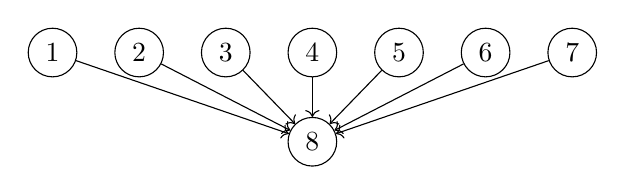
\begin{tikzpicture}[yscale=-1.03,scale=1.1]
	\node [fill=white, draw=black, shape=circle, minimum size=6mm] (1) at (0, 1) {8};
	
	%\node [fill=white, draw=black, shape=circle, minimum size=6mm] (2) at (-4, 0) {2};
	\node [fill=white, draw=black, shape=circle, minimum size=6mm] (3) at (-3, 0) {1};
	\node [fill=white, draw=black, shape=circle, minimum size=6mm] (4) at (-2, 0) {2};
	\node [fill=white, draw=black, shape=circle, minimum size=6mm] (5) at (-1, 0) {3};
	\node [fill=white, draw=black, shape=circle, minimum size=6mm] (6) at (0, 0) {4};
	\node [fill=white, draw=black, shape=circle, minimum size=6mm] (7) at (1, 0) {5};
	\node [fill=white, draw=black, shape=circle, minimum size=6mm] (8) at (2, 0) {6};
	\node [fill=white, draw=black, shape=circle, minimum size=6mm] (9) at (3, 0) {7};
	%\node [fill=white, draw=black, shape=circle, minimum size=6mm] (10) at (4, 0) {10};

	
	%\draw [fill=none, ->] (2) to (1);
	\draw [fill=none, ->] (3) to (1);
	\draw [fill=none, ->] (4) to (1);
	\draw [fill=none, ->] (5) to (1);
	\draw [fill=none, ->] (6) to (1);
	\draw [fill=none, ->] (7) to (1);
	\draw [fill=none, ->] (8) to (1);
	\draw [fill=none, ->] (9) to (1);
	%\draw [fill=none, ->] (10) to (1);
\end{tikzpicture}
\caption[An example DAG for conjoined small-hard problems]{An example DAG for conjoined small-hard problems, where disjoint subproblems are processed in parallel and their solutions joined together at the final node}\label{fig:dag_example4315}
\end{figure}


The run-time of search on  super-problems with varying numbers of subproblems, in different computational environments where we vary the number of available cores, is shown in Figures~\ref{fig:performance_graph1}~and~\ref{fig:performance_graph2}.
%%
From Figure~\ref{fig:performance_graph1} we can see that as the number of subproblems increases the time it takes \dagster\ to solve the problem as a fraction of the time it takes the baseline CDCL procedure, \tinisat, to solve the problem decreases -- i.e. \dagster\ is significantly faster.
Particularly, it is possible to note that the trend-line is approximately hyperbolic, indicating that the computational overhead of using \dagster\ goes to zero as the number of subproblems increases.
Also, the speed of \dagster\ is pseudo-linearly increasing for large numbers of subproblems from figure \ref{fig:performance_graph2} which is expected.
The reader should also not that here, \dagster\ is solving a more difficult problem compared to the CDCL baseline.
It has to find the one satisfying valuable, and then further prove that no further solutions exists.

We also notice that increasing the number of cores available to \dagster\ solving the problem increases performance, but only upto a certain point.
Particularly it was noticed that $64$ cores performed significantly worse than $32$ cores.
This measurement of degrading performance is something we shall investigate in due course, and is likely due to the experimental host being oversubscribed at the time we took the measurement. 

The invocation to run the above experiment is to be found by executed the following command within the code repository:

\begin{verbatim}
python3 ~/summer1819/Benchmarks/cnf_concatenator/run.py
\end{verbatim}

Experimenting with with small-hard problems in parallel we were able to verify that \dagster\ offers significant parallel advantage, as is expected by its design.

   \begin{figure}[]
        \centering
		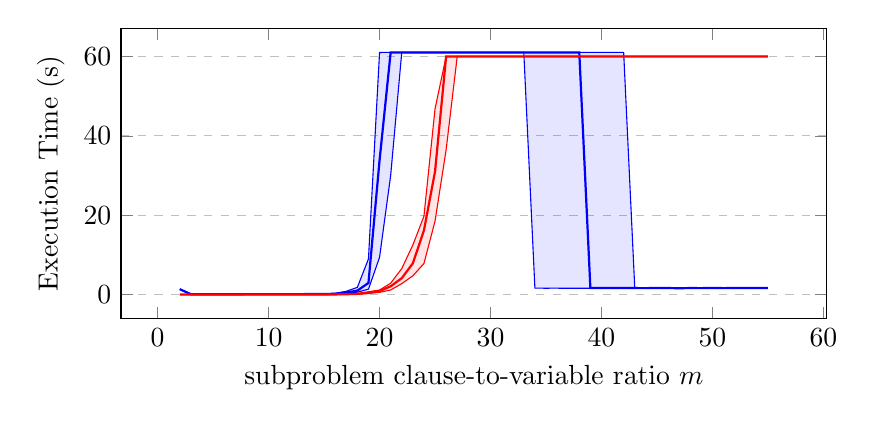
\begin{tikzpicture}
		\begin{axis}[
			title={},
			xlabel={subproblem clause-to-variable ratio $m$},
			ylabel={Execution Time (s)},
			%xmin=0, xmax=0.25,
			%ymin=10.00, ymax=100000.00,
			%ymode=log,
			%xtick={0,0.05,0.1,0.15,0.2,0.25},
			%ytick={0,20,40,60,80,100},
			%yticklabel=$\pgfmathprintnumber{\tick}\%$,
			legend pos=south west,
			ymajorgrids=true,
			grid style=dashed,
			xticklabel style={/pgf/number format/fixed},
			width = 300,
			height = 150
		]


		\addplot[name path=f1,color=blue,line width=0.4pt] coordinates {
(2,1.3527034521102905)(3,0.09176099300384521)(4,0.09236204624176025)(5,0.09132146835327148)(6,0.09429752826690674)(7,0.09694063663482666)(8,0.11464154720306396)(9,0.11499607563018799)(10,0.1169133186340332)(11,0.11847519874572754)(12,0.12066256999969482)(13,0.12117254734039307)(14,0.12333226203918457)(15,0.13137030601501465)(16,0.16925442218780518)(17,0.3175164461135864)(18,0.6166036128997803)(19,1.3711258172988892)(20,9.400351643562317)(21,29.993253231048584)(22,61.00600075721741)(23,61.00604474544525)(24,61.00608855485916)(25,61.006143391132355)(26,61.006144523620605)(27,61.006110310554504)(28,61.00610476732254)(29,61.006164610385895)(30,61.00612485408783)(31,61.00609648227692)(32,61.00603848695755)(33,61.00610190629959)(34,1.6209341883659363)(35,1.6125808358192444)(36,1.6190196871757507)(37,1.5884765982627869)(38,1.6029763221740723)(39,1.6009960174560547)(40,1.5929163694381714)(41,1.5890370607376099)(42,1.5909844636917114)(43,1.5938313007354736)(44,1.5936198830604553)(45,1.5897762179374695)(46,1.5980766415596008)(47,1.5893039107322693)(48,1.6110384464263916)(49,1.6085428595542908)(50,1.6058598756790161)(51,1.6078521609306335)(52,1.6065120697021484)(53,1.6256402134895325)(54,1.626099705696106)(55,1.6245319843292236)
			}node[pos=0.8](endofplotsquare){} ;
		\addplot[color=blue,line width=0.8pt] coordinates {
(2,1.3614459037780762)(3,0.09326696395874023)(4,0.0951998233795166)(5,0.09443187713623047)(6,0.09698915481567383)(7,0.10982441902160645)(8,0.1189274787902832)(9,0.11959409713745117)(10,0.12096667289733887)(11,0.12102866172790527)(12,0.12321853637695312)(13,0.1243593692779541)(14,0.12966251373291016)(15,0.1486351490020752)(16,0.21170949935913086)(17,0.5399208068847656)(18,1.0046255588531494)(19,2.9330649375915527)(20,33.83585262298584)(21,61.006205320358276)(22,61.00628936290741)(23,61.00627958774567)(24,61.00637245178223)(25,61.006428360939026)(26,61.00637710094452)(27,61.00629651546478)(28,61.0062518119812)(29,61.00653564929962)(30,61.006577134132385)(31,61.006420850753784)(32,61.00664949417114)(33,61.006407499313354)(34,61.006426215171814)(35,61.006422996520996)(36,61.00623905658722)(37,61.00621461868286)(38,61.00621461868286)(39,1.6477763652801514)(40,1.6525676250457764)(41,1.6660830974578857)(42,1.644205093383789)(43,1.640013575553894)(44,1.630387306213379)(45,1.6524988412857056)(46,1.6457465887069702)(47,1.6131200790405273)(48,1.6458690166473389)(49,1.6322563886642456)(50,1.6606208086013794)(51,1.6331430673599243)(52,1.6514649391174316)(53,1.6669789552688599)(54,1.662269949913025)(55,1.6571600437164307)
			}node[pos=0.8](endofplotsquare){} ;
		\addplot[name path=f2,color=blue,line width=0.4pt] coordinates {
(2,1.3697444200515747)(3,0.09605276584625244)(4,0.09871494770050049)(5,0.0977625846862793)(6,0.10048854351043701)(7,0.11725211143493652)(8,0.12633860111236572)(9,0.1230776309967041)(10,0.12476563453674316)(11,0.12495827674865723)(12,0.1258915662765503)(13,0.12760019302368164)(14,0.13661205768585205)(15,0.16915571689605713)(16,0.32639896869659424)(17,0.8259114027023315)(18,1.8294086456298828)(19,8.992531776428223)(20,61.006160855293274)(21,61.006909012794495)(22,61.0068975687027)(23,61.00688046216965)(24,61.006865203380585)(25,61.00694364309311)(26,61.0067183971405)(27,61.00685328245163)(28,61.006638169288635)(29,61.00702488422394)(30,61.007180869579315)(31,61.00738716125488)(32,61.00726270675659)(33,61.007057785987854)(34,61.00727742910385)(35,61.0072203874588)(36,61.00772112607956)(37,61.0065820813179)(38,61.00792121887207)(39,61.00731736421585)(40,61.00646638870239)(41,61.00753968954086)(42,61.007122218608856)(43,1.6911166310310364)(44,1.6843940615653992)(45,1.6967138051986694)(46,1.6964040994644165)(47,1.6678423285484314)(48,1.7020439505577087)(49,1.6689872741699219)(50,1.7089079022407532)(51,1.6987597346305847)(52,1.7034250497817993)(53,1.6990136504173279)(54,1.7044062614440918)(55,1.7066537737846375)
			}node[pos=0.8](endofplotsquare){} ;
		\addplot[name path=f3,color=red,line width=0.4pt] coordinates {
(2,0.0046389102935791016)(3,0.0040814876556396484)(4,0.004398822784423828)(5,0.0046138763427734375)(6,0.005382895469665527)(7,0.005793333053588867)(8,0.0064470767974853516)(9,0.006873011589050293)(10,0.0073473453521728516)(11,0.007998824119567871)(12,0.008495688438415527)(13,0.009410500526428223)(14,0.011755228042602539)(15,0.01363980770111084)(16,0.02518320083618164)(17,0.04995083808898926)(18,0.13091230392456055)(19,0.30581045150756836)(20,0.571260929107666)(21,1.1591084003448486)(22,2.7681276202201843)(23,4.739260315895081)(24,7.829183459281921)(25,18.509818077087402)(26,36.49925708770752)(27,60.00207221508026)(28,60.002069771289825)(29,60.0021196603775)(30,60.00206017494202)(31,60.002059519290924)(32,60.00207161903381)(33,60.00206017494202)(34,60.00205045938492)(35,60.00203728675842)(36,60.00203835964203)(37,60.00205773115158)(38,60.002051174640656)(39,60.00204664468765)(40,60.002042174339294)(41,60.0020307302475)(42,60.00202852487564)(43,60.002033829689026)(44,60.002032697200775)(45,60.00203174352646)(46,60.00205159187317)(47,60.00204926729202)(48,60.002038061618805)(49,60.00207084417343)(50,60.002087354660034)(51,60.00210380554199)(52,60.00211697816849)(53,60.002116084098816)(54,60.00214123725891)(55,60.002137184143066)
			}node[pos=0.8](endofplotsquare){} ;
		\addplot[color=red,line width=0.8pt] coordinates {
(2,0.00505518913269043)(3,0.0045032501220703125)(4,0.0048828125)(5,0.005078315734863281)(6,0.005706310272216797)(7,0.006450176239013672)(8,0.0070743560791015625)(9,0.007384777069091797)(10,0.008163928985595703)(11,0.008799552917480469)(12,0.009170055389404297)(13,0.010346651077270508)(14,0.013486385345458984)(15,0.017902374267578125)(16,0.046679019927978516)(17,0.09327006340026855)(18,0.18178248405456543)(19,0.4199967384338379)(20,0.8862345218658447)(21,2.0927345752716064)(22,4.138214588165283)(23,7.871921539306641)(24,16.18044602870941)(25,31.001109719276428)(26,60.00212013721466)(27,60.00220429897308)(28,60.00220572948456)(29,60.00222420692444)(30,60.002148389816284)(31,60.00211811065674)(32,60.00212383270264)(33,60.00211143493652)(34,60.00210201740265)(35,60.002113699913025)(36,60.002126812934875)(37,60.00210404396057)(38,60.00210785865784)(39,60.00207710266113)(40,60.002108693122864)(41,60.00206744670868)(42,60.00207817554474)(43,60.00208342075348)(44,60.002084851264954)(45,60.002066135406494)(46,60.002139925956726)(47,60.00210452079773)(48,60.00208902359009)(49,60.00210666656494)(50,60.00214326381683)(51,60.00219964981079)(52,60.00221276283264)(53,60.00220715999603)(54,60.00220715999603)(55,60.002225279808044)
			}node[pos=0.8](endofplotsquare){} ;
		\addplot[name path=f4,color=red,line width=0.4pt] coordinates {
(2,0.005779862403869629)(3,0.005020618438720703)(4,0.00543057918548584)(5,0.0056198835372924805)(6,0.006289362907409668)(7,0.007857441902160645)(8,0.015705585479736328)(9,0.007815957069396973)(10,0.008703947067260742)(11,0.009836196899414062)(12,0.010218381881713867)(13,0.011949896812438965)(14,0.017240524291992188)(15,0.024730563163757324)(16,0.07063519954681396)(17,0.12457525730133057)(18,0.29529857635498047)(19,0.7256525754928589)(20,1.1562894582748413)(21,2.8747419118881226)(22,6.56018340587616)(23,12.49211984872818)(24,19.739576280117035)(25,46.802177250385284)(26,60.00236755609512)(27,60.00236427783966)(28,60.00233578681946)(29,60.00232398509979)(30,60.00224858522415)(31,60.002268612384796)(32,60.002237141132355)(33,60.00219076871872)(34,60.00216329097748)(35,60.0021830201149)(36,60.00219541788101)(37,60.002164125442505)(38,60.002209544181824)(39,60.00213420391083)(40,60.00222772359848)(41,60.00217932462692)(42,60.00219810009003)(43,60.00217795372009)(44,60.00216448307037)(45,60.002122938632965)(46,60.00221198797226)(47,60.00216209888458)(48,60.002180099487305)(49,60.00221639871597)(50,60.00225609540939)(51,60.002464056015015)(52,60.00229650735855)(53,60.00232136249542)(54,60.00238847732544)(55,60.00235724449158)
			}node[pos=0.8](endofplotsquare){} ;


\addplot [
        thick,
        color=blue,
        fill=blue, 
        fill opacity=0.1
    ]
    fill between[
        of=f1 and f2
    ];
\addplot [
        thick,
        color=red,
        fill=red, 
        fill opacity=0.1
    ]
    fill between[
        of=f3 and f4
    ];

		\end{axis}
		\end{tikzpicture}
		%\vspace{-18pt}
		\caption[Runtime performance for random structured problems with few overlapping variables]{Runtime performance (medians and interquartile ranges) of \textsc{Dagster} (as blue) and \textsc{Minisat} (as red) for structured problems given by algorithm \ref{algorithm1} with few overlapping variables ($s=100,p=5,s=4,c=5$)}
		\label{fig:performance_graph1}
    \end{figure}

   \begin{figure}[h]
        \centering
		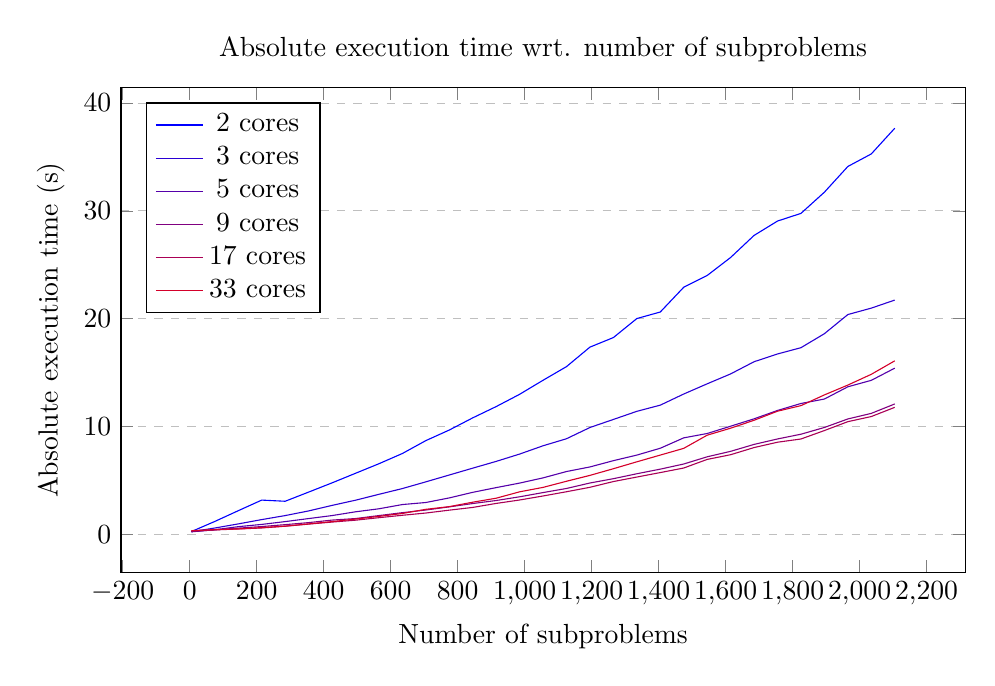
\begin{tikzpicture}
		\begin{axis}[
			title={Absolute execution time wrt. number of subproblems},
			xlabel={Number of subproblems},
			ylabel={Absolute execution time (s)},
			%xmin=0, xmax=0.25,
			%ymin=10.00, ymax=100000.00,
			%ymode=log,
			%xtick={0,0.05,0.1,0.15,0.2,0.25},
			%ytick={0,20,40,60,80,100},
			%yticklabel=$\pgfmathprintnumber{\tick}\%$,
			legend pos=north west,
			ymajorgrids=true,
			grid style=dashed,
			xticklabel style={/pgf/number format/fixed},
			width = 350,
			height = 220
		]




\addplot[color=red!0.0!blue,line width=0.4pt] coordinates {
(5,0.2362961769104004)(75,1.1755552291870117)(145,2.173146963119507)(215,3.157050848007202)(285,3.0487685203552246)(355,3.8985092639923096)(425,4.755660533905029)(495,5.643772602081299)(565,6.531620502471924)(635,7.4814841747283936)(705,8.676511764526367)(775,9.6584312915802)(845,10.788349628448486)(915,11.835201978683472)(985,12.97413420677185)(1055,14.27720332145691)(1125,15.543988466262817)(1195,17.353617668151855)(1265,18.240656852722168)(1335,20.005002737045288)(1405,20.61204719543457)(1475,22.910298585891724)(1545,24.000704765319824)(1615,25.671855211257935)(1685,27.71861171722412)(1755,29.05149006843567)(1825,29.763449668884277)(1895,31.731281280517578)(1965,34.11725568771362)(2035,35.28141164779663)(2105,37.66511368751526)
}node[pos=0.8](endofplotsquare){} ;
\addlegendentry{2 cores}
\addplot[color=red!16.666666666666668!blue,line width=0.4pt] coordinates {
(5,0.22471952438354492)(75,0.5662057399749756)(145,0.9474582672119141)(215,1.348191499710083)(285,1.7202212810516357)(355,2.151851177215576)(425,2.665273904800415)(495,3.1462738513946533)(565,3.693495988845825)(635,4.227936029434204)(705,4.85132622718811)(775,5.485703945159912)(845,6.121047019958496)(915,6.748381614685059)(985,7.428805828094482)(1055,8.197736501693726)(1125,8.851788997650146)(1195,9.894617795944214)(1265,10.641643524169922)(1335,11.394659757614136)(1405,11.9686861038208)(1475,13.001048803329468)(1545,13.947997093200684)(1615,14.866320371627808)(1685,15.998363256454468)(1755,16.718042373657227)(1825,17.30029273033142)(1895,18.59991478919983)(1965,20.375839233398438)(2035,20.972047805786133)(2105,21.719709873199463)
}node[pos=0.8](endofplotsquare){} ;
\addlegendentry{3 cores}
\addplot[color=red!33.333333333333336!blue,line width=0.4pt] coordinates {
(5,0.21304702758789062)(75,0.40426206588745117)(145,0.6919465065002441)(215,0.8999366760253906)(285,1.161741018295288)(355,1.4429419040679932)(425,1.7209069728851318)(495,2.0703799724578857)(565,2.3511414527893066)(635,2.743969202041626)(705,2.93356990814209)(775,3.3594651222229004)(845,3.8780977725982666)(915,4.315030574798584)(985,4.735558748245239)(1055,5.218811988830566)(1125,5.80847954750061)(1195,6.234036207199097)(1265,6.816247940063477)(1335,7.3333940505981445)(1405,7.969827890396118)(1475,8.932463884353638)(1545,9.336983680725098)(1615,10.014135122299194)(1685,10.699220180511475)(1755,11.475051641464233)(1825,12.123208999633789)(1895,12.535733938217163)(1965,13.671947479248047)(2035,14.27146577835083)(2105,15.399876117706299)
}node[pos=0.8](endofplotsquare){} ;
\addlegendentry{5 cores}
\addplot[color=red!50.0!blue,line width=0.4pt] coordinates {
(5,0.23718547821044922)(75,0.39684247970581055)(145,0.5541701316833496)(215,0.7023584842681885)(285,0.8778998851776123)(355,1.0677170753479004)(425,1.3016605377197266)(495,1.4439446926116943)(565,1.7219109535217285)(635,1.9910361766815186)(705,2.2353708744049072)(775,2.528398036956787)(845,2.8381338119506836)(915,3.1183969974517822)(985,3.463233470916748)(1055,3.8552088737487793)(1125,4.2365453243255615)(1195,4.743107080459595)(1265,5.144285202026367)(1335,5.602648973464966)(1405,6.029825448989868)(1475,6.506726264953613)(1545,7.1754631996154785)(1615,7.681975603103638)(1685,8.325080871582031)(1755,8.830584049224854)(1825,9.272136449813843)(1895,9.895843505859375)(1965,10.687816381454468)(2035,11.204007387161255)(2105,12.079752206802368)
}node[pos=0.8](endofplotsquare){} ;
\addlegendentry{9 cores}
\addplot[color=red!66.66666666666667!blue,line width=0.4pt] coordinates {
(5,0.2891275882720947)(75,0.3904001712799072)(145,0.4757850170135498)(215,0.5699207782745361)(285,0.7323768138885498)(355,0.9299347400665283)(425,1.118117332458496)(495,1.292304515838623)(565,1.525442361831665)(635,1.748434066772461)(705,1.957042932510376)(775,2.223759651184082)(845,2.476705551147461)(915,2.8478481769561768)(985,3.1665890216827393)(1055,3.5390067100524902)(1125,3.9331343173980713)(1195,4.345015525817871)(1265,4.87886118888855)(1335,5.296087265014648)(1405,5.711444616317749)(1475,6.134087324142456)(1545,6.932433128356934)(1615,7.369121313095093)(1685,8.03252911567688)(1755,8.528788566589355)(1825,8.827685832977295)(1895,9.611763715744019)(1965,10.435662269592285)(2035,10.911863565444946)(2105,11.763577699661255)
}node[pos=0.8](endofplotsquare){} ;
\addlegendentry{17 cores}
\addplot[color=red!83.33333333333333!blue,line width=0.4pt] coordinates {
(5,0.32294368743896484)(75,0.41986513137817383)(145,0.48233509063720703)(215,0.6048417091369629)(285,0.7414553165435791)(355,0.9482111930847168)(425,1.16239333152771)(495,1.3949286937713623)(565,1.645319938659668)(635,1.9154088497161865)(705,2.3016510009765625)(775,2.5509541034698486)(845,2.9621360301971436)(915,3.3325388431549072)(985,3.925122022628784)(1055,4.336254119873047)(1125,4.905707359313965)(1195,5.449917554855347)(1265,6.069330453872681)(1335,6.710622310638428)(1405,7.333817720413208)(1475,7.9586451053619385)(1545,9.180939674377441)(1615,9.829682111740112)(1685,10.564534664154053)(1755,11.407931804656982)(1825,11.923769474029541)(1895,12.91983437538147)(1965,13.831814765930176)(2035,14.831673383712769)(2105,16.079890727996826)
}node[pos=0.8](endofplotsquare){} ;
\addlegendentry{33 cores}



		\end{axis}
		\end{tikzpicture}
		%\vspace{-18pt}
		\caption[Absolute execution time wrt. number small-hard subproblems]{Runtime on paralell small-hard subproblems, for different numbers of cores and subprobems}
		\label{fig:performance_graph2}
    \end{figure}


\clearpage


\section{A Large Satisfiable Problem - Pentominoes}

A tiling problem was extended as a benchmark for \dagster\ from a recreational puzzle solving youtube channel\footnote{Cracking the Cryptic, youtube video: \url{youtube.com/watch?v=S2aN-s3hG6Y}}, as shown in Figure \ref{fig:pentomino_puzzle1}, where the challenge is to fill a grid with Pentominoes (5 connected blocks) such that no pentomino crosses a boldened black line, and that no pentominoes of the same shape (counting reflections/rotations) touch each other.


\begin{figure}[h]
\centering
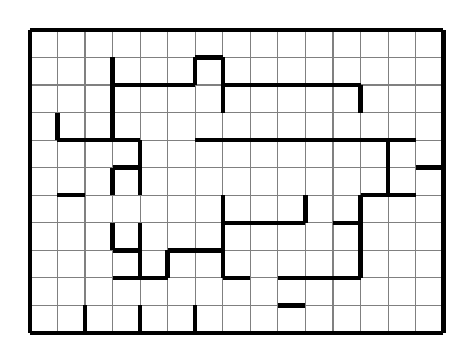
\begin{tikzpicture}[xscale=0.35, yscale=-0.35]
\draw[gray,thin] (0,0)--(0,11);
\draw[gray,thin] (1,0)--(1,11);
\draw[gray,thin] (2,0)--(2,11);
\draw[gray,thin] (3,0)--(3,11);
\draw[gray,thin] (4,0)--(4,11);
\draw[gray,thin] (5,0)--(5,11);
\draw[gray,thin] (6,0)--(6,11);
\draw[gray,thin] (7,0)--(7,11);
\draw[gray,thin] (8,0)--(8,11);
\draw[gray,thin] (9,0)--(9,11);
\draw[gray,thin] (10,0)--(10,11);
\draw[gray,thin] (11,0)--(11,11);
\draw[gray,thin] (12,0)--(12,11);
\draw[gray,thin] (13,0)--(13,11);
\draw[gray,thin] (14,0)--(14,11);
\draw[gray,thin] (0,0)--(15,0);
\draw[gray,thin] (0,1)--(15,1);
\draw[gray,thin] (0,2)--(15,2);
\draw[gray,thin] (0,3)--(15,3);
\draw[gray,thin] (0,4)--(15,4);
\draw[gray,thin] (0,5)--(15,5);
\draw[gray,thin] (0,6)--(15,6);
\draw[gray,thin] (0,7)--(15,7);
\draw[gray,thin] (0,8)--(15,8);
\draw[gray,thin] (0,9)--(15,9);
\draw[gray,thin] (0,10)--(15,10);
\draw[ultra thick] (6,1)--(7,1);
\draw[ultra thick] (3,1)--(3,2);
\draw[ultra thick] (3,2)--(4,2);
\draw[ultra thick] (4,2)--(5,2);
\draw[ultra thick] (6,1)--(6,2);
\draw[ultra thick] (5,2)--(6,2);
\draw[ultra thick] (7,1)--(7,2);
\draw[ultra thick] (7,2)--(8,2);
\draw[ultra thick] (8,2)--(9,2);
\draw[ultra thick] (9,2)--(10,2);
\draw[ultra thick] (10,2)--(11,2);
\draw[ultra thick] (11,2)--(12,2);
\draw[ultra thick] (3,2)--(3,3);
\draw[ultra thick] (7,2)--(7,3);
\draw[ultra thick] (12,2)--(12,3);
\draw[ultra thick] (1,3)--(1,4);
\draw[ultra thick] (1,4)--(2,4);
\draw[ultra thick] (3,3)--(3,4);
\draw[ultra thick] (2,4)--(3,4);
\draw[ultra thick] (3,4)--(4,4);
\draw[ultra thick] (6,4)--(7,4);
\draw[ultra thick] (7,4)--(8,4);
\draw[ultra thick] (8,4)--(9,4);
\draw[ultra thick] (9,4)--(10,4);
\draw[ultra thick] (10,4)--(11,4);
\draw[ultra thick] (11,4)--(12,4);
\draw[ultra thick] (12,4)--(13,4);
\draw[ultra thick] (13,4)--(14,4);
\draw[ultra thick] (4,4)--(4,5);
\draw[ultra thick] (3,5)--(4,5);
\draw[ultra thick] (13,4)--(13,5);
\draw[ultra thick] (14,5)--(15,5);
\draw[ultra thick] (1,6)--(2,6);
\draw[ultra thick] (3,5)--(3,6);
\draw[ultra thick] (4,5)--(4,6);
\draw[ultra thick] (13,5)--(13,6);
\draw[ultra thick] (12,6)--(13,6);
\draw[ultra thick] (13,6)--(14,6);
\draw[ultra thick] (7,6)--(7,7);
\draw[ultra thick] (7,7)--(8,7);
\draw[ultra thick] (8,7)--(9,7);
\draw[ultra thick] (10,6)--(10,7);
\draw[ultra thick] (9,7)--(10,7);
\draw[ultra thick] (12,6)--(12,7);
\draw[ultra thick] (11,7)--(12,7);
\draw[ultra thick] (3,7)--(3,8);
\draw[ultra thick] (4,7)--(4,8);
\draw[ultra thick] (3,8)--(4,8);
\draw[ultra thick] (5,8)--(6,8);
\draw[ultra thick] (7,7)--(7,8);
\draw[ultra thick] (6,8)--(7,8);
\draw[ultra thick] (12,7)--(12,8);
\draw[ultra thick] (4,8)--(4,9);
\draw[ultra thick] (3,9)--(4,9);
\draw[ultra thick] (5,8)--(5,9);
\draw[ultra thick] (4,9)--(5,9);
\draw[ultra thick] (7,8)--(7,9);
\draw[ultra thick] (7,9)--(8,9);
\draw[ultra thick] (9,9)--(10,9);
\draw[ultra thick] (10,9)--(11,9);
\draw[ultra thick] (12,8)--(12,9);
\draw[ultra thick] (11,9)--(12,9);
\draw[ultra thick] (9,10)--(10,10);
\draw[ultra thick] (2,10)--(2,11);
\draw[ultra thick] (4,10)--(4,11);
\draw[ultra thick] (6,10)--(6,11);
\draw[ultra thick] (0,0)--(0,11);
\draw[ultra thick] (0,0)--(15,0);
\draw[ultra thick] (15,11)--(0,11);
\draw[ultra thick] (15,11)--(15,0);
\end{tikzpicture}
\caption{A Pentomino puzzle featured on youtube channel `Cracking the Cryptic'}\label{fig:pentomino_puzzle1}
\end{figure}


A generator of these kind of problems was coded to randomly generate hard 15x15 pentomino problems, involving a process of:
\begin{enumerate}
\item	Randomly filling a 15x15 grid with pentominoes
\item	Bolden the outline of those pentominoes, and removing them
\item	Iteratively remove a random boldened line segments while the puzzle is uniquely solvable, until no more such removals are possible.
\end{enumerate}

This process was shown to become prohibitively slow to generate problems larger than 25x25, and so to generate bigger pentomino problems these 15x15 pentomino problems were cascaded side-by-side together in a grid pattern, such as shown in Figure \ref{subproblem2}.
In this way, the grid of pentomino problems constitutes a larger problem which has logically distinct parts and where each subproblem is logically related only to its immediate neighbours: above, below, left and right; and because every pentomino subproblem is uniquely solvable then also this larger pentomino problem is also uniquely solvable.

For these large pentomino problems a DAG would be generated embodying a solution process of solving from the top left diagonally through to the bottom right, as shown in Figure \ref{fig:dag_example1215}.
In these particular problems the size of the grid of 15x15 pentomino subproblems would determine the maximum branching of the parallel process and thus the efficiency of the solving in parallel.

\begin{figure}[h]
\centering
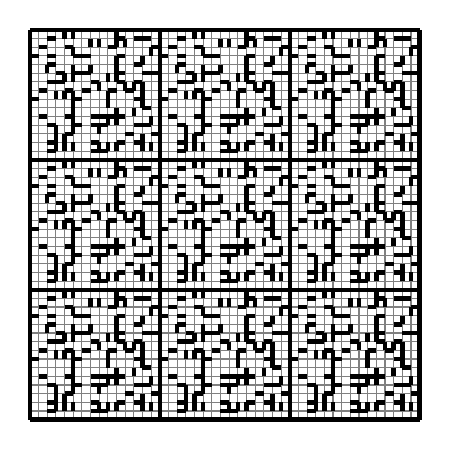
\begin{tikzpicture}[scale=0.11]
\draw[gray,thin] (0,0)--(0,45);
\draw[gray,thin] (1,0)--(1,45);
\draw[gray,thin] (2,0)--(2,45);
\draw[gray,thin] (3,0)--(3,45);
\draw[gray,thin] (4,0)--(4,45);
\draw[gray,thin] (5,0)--(5,45);
\draw[gray,thin] (6,0)--(6,45);
\draw[gray,thin] (7,0)--(7,45);
\draw[gray,thin] (8,0)--(8,45);
\draw[gray,thin] (9,0)--(9,45);
\draw[gray,thin] (10,0)--(10,45);
\draw[gray,thin] (11,0)--(11,45);
\draw[gray,thin] (12,0)--(12,45);
\draw[gray,thin] (13,0)--(13,45);
\draw[gray,thin] (14,0)--(14,45);
\draw[gray,thin] (15,0)--(15,45);
\draw[gray,thin] (16,0)--(16,45);
\draw[gray,thin] (17,0)--(17,45);
\draw[gray,thin] (18,0)--(18,45);
\draw[gray,thin] (19,0)--(19,45);
\draw[gray,thin] (20,0)--(20,45);
\draw[gray,thin] (21,0)--(21,45);
\draw[gray,thin] (22,0)--(22,45);
\draw[gray,thin] (23,0)--(23,45);
\draw[gray,thin] (24,0)--(24,45);
\draw[gray,thin] (25,0)--(25,45);
\draw[gray,thin] (26,0)--(26,45);
\draw[gray,thin] (27,0)--(27,45);
\draw[gray,thin] (28,0)--(28,45);
\draw[gray,thin] (29,0)--(29,45);
\draw[gray,thin] (30,0)--(30,45);
\draw[gray,thin] (31,0)--(31,45);
\draw[gray,thin] (32,0)--(32,45);
\draw[gray,thin] (33,0)--(33,45);
\draw[gray,thin] (34,0)--(34,45);
\draw[gray,thin] (35,0)--(35,45);
\draw[gray,thin] (36,0)--(36,45);
\draw[gray,thin] (37,0)--(37,45);
\draw[gray,thin] (38,0)--(38,45);
\draw[gray,thin] (39,0)--(39,45);
\draw[gray,thin] (40,0)--(40,45);
\draw[gray,thin] (41,0)--(41,45);
\draw[gray,thin] (42,0)--(42,45);
\draw[gray,thin] (43,0)--(43,45);
\draw[gray,thin] (44,0)--(44,45);
\draw[gray,thin] (0,0)--(45,0);
\draw[gray,thin] (0,1)--(45,1);
\draw[gray,thin] (0,2)--(45,2);
\draw[gray,thin] (0,3)--(45,3);
\draw[gray,thin] (0,4)--(45,4);
\draw[gray,thin] (0,5)--(45,5);
\draw[gray,thin] (0,6)--(45,6);
\draw[gray,thin] (0,7)--(45,7);
\draw[gray,thin] (0,8)--(45,8);
\draw[gray,thin] (0,9)--(45,9);
\draw[gray,thin] (0,10)--(45,10);
\draw[gray,thin] (0,11)--(45,11);
\draw[gray,thin] (0,12)--(45,12);
\draw[gray,thin] (0,13)--(45,13);
\draw[gray,thin] (0,14)--(45,14);
\draw[gray,thin] (0,15)--(45,15);
\draw[gray,thin] (0,16)--(45,16);
\draw[gray,thin] (0,17)--(45,17);
\draw[gray,thin] (0,18)--(45,18);
\draw[gray,thin] (0,19)--(45,19);
\draw[gray,thin] (0,20)--(45,20);
\draw[gray,thin] (0,21)--(45,21);
\draw[gray,thin] (0,22)--(45,22);
\draw[gray,thin] (0,23)--(45,23);
\draw[gray,thin] (0,24)--(45,24);
\draw[gray,thin] (0,25)--(45,25);
\draw[gray,thin] (0,26)--(45,26);
\draw[gray,thin] (0,27)--(45,27);
\draw[gray,thin] (0,28)--(45,28);
\draw[gray,thin] (0,29)--(45,29);
\draw[gray,thin] (0,30)--(45,30);
\draw[gray,thin] (0,31)--(45,31);
\draw[gray,thin] (0,32)--(45,32);
\draw[gray,thin] (0,33)--(45,33);
\draw[gray,thin] (0,34)--(45,34);
\draw[gray,thin] (0,35)--(45,35);
\draw[gray,thin] (0,36)--(45,36);
\draw[gray,thin] (0,37)--(45,37);
\draw[gray,thin] (0,38)--(45,38);
\draw[gray,thin] (0,39)--(45,39);
\draw[gray,thin] (0,40)--(45,40);
\draw[gray,thin] (0,41)--(45,41);
\draw[gray,thin] (0,42)--(45,42);
\draw[gray,thin] (0,43)--(45,43);
\draw[gray,thin] (0,44)--(45,44);
\draw[ultra thick] (2,1)--(3,1);
\draw[ultra thick] (7,1)--(8,1);
\draw[ultra thick] (8,1)--(9,1);
\draw[ultra thick] (15,0)--(15,1);
\draw[ultra thick] (17,1)--(18,1);
\draw[ultra thick] (22,1)--(23,1);
\draw[ultra thick] (23,1)--(24,1);
\draw[ultra thick] (30,0)--(30,1);
\draw[ultra thick] (32,1)--(33,1);
\draw[ultra thick] (37,1)--(38,1);
\draw[ultra thick] (38,1)--(39,1);
\draw[ultra thick] (45,0)--(45,1);
\draw[ultra thick] (3,1)--(3,2);
\draw[ultra thick] (2,2)--(3,2);
\draw[ultra thick] (4,1)--(4,2);
\draw[ultra thick] (5,1)--(5,2);
\draw[ultra thick] (8,1)--(8,2);
\draw[ultra thick] (7,2)--(8,2);
\draw[ultra thick] (9,1)--(9,2);
\draw[ultra thick] (10,1)--(10,2);
\draw[ultra thick] (10,2)--(11,2);
\draw[ultra thick] (13,1)--(13,2);
\draw[ultra thick] (12,2)--(13,2);
\draw[ultra thick] (14,1)--(14,2);
\draw[ultra thick] (15,1)--(15,2);
\draw[ultra thick] (18,1)--(18,2);
\draw[ultra thick] (17,2)--(18,2);
\draw[ultra thick] (19,1)--(19,2);
\draw[ultra thick] (20,1)--(20,2);
\draw[ultra thick] (23,1)--(23,2);
\draw[ultra thick] (22,2)--(23,2);
\draw[ultra thick] (24,1)--(24,2);
\draw[ultra thick] (25,1)--(25,2);
\draw[ultra thick] (25,2)--(26,2);
\draw[ultra thick] (28,1)--(28,2);
\draw[ultra thick] (27,2)--(28,2);
\draw[ultra thick] (29,1)--(29,2);
\draw[ultra thick] (30,1)--(30,2);
\draw[ultra thick] (33,1)--(33,2);
\draw[ultra thick] (32,2)--(33,2);
\draw[ultra thick] (34,1)--(34,2);
\draw[ultra thick] (35,1)--(35,2);
\draw[ultra thick] (38,1)--(38,2);
\draw[ultra thick] (37,2)--(38,2);
\draw[ultra thick] (39,1)--(39,2);
\draw[ultra thick] (40,1)--(40,2);
\draw[ultra thick] (40,2)--(41,2);
\draw[ultra thick] (43,1)--(43,2);
\draw[ultra thick] (42,2)--(43,2);
\draw[ultra thick] (44,1)--(44,2);
\draw[ultra thick] (45,1)--(45,2);
\draw[ultra thick] (3,2)--(3,3);
\draw[ultra thick] (4,2)--(4,3);
\draw[ultra thick] (4,3)--(5,3);
\draw[ultra thick] (11,3)--(12,3);
\draw[ultra thick] (13,2)--(13,3);
\draw[ultra thick] (15,2)--(15,3);
\draw[ultra thick] (14,3)--(15,3);
\draw[ultra thick] (18,2)--(18,3);
\draw[ultra thick] (19,2)--(19,3);
\draw[ultra thick] (19,3)--(20,3);
\draw[ultra thick] (26,3)--(27,3);
\draw[ultra thick] (28,2)--(28,3);
\draw[ultra thick] (30,2)--(30,3);
\draw[ultra thick] (29,3)--(30,3);
\draw[ultra thick] (33,2)--(33,3);
\draw[ultra thick] (34,2)--(34,3);
\draw[ultra thick] (34,3)--(35,3);
\draw[ultra thick] (41,3)--(42,3);
\draw[ultra thick] (43,2)--(43,3);
\draw[ultra thick] (45,2)--(45,3);
\draw[ultra thick] (44,3)--(45,3);
\draw[ultra thick] (3,3)--(3,4);
\draw[ultra thick] (2,4)--(3,4);
\draw[ultra thick] (5,3)--(5,4);
\draw[ultra thick] (5,4)--(6,4);
\draw[ultra thick] (8,3)--(8,4);
\draw[ultra thick] (7,4)--(8,4);
\draw[ultra thick] (8,4)--(9,4);
\draw[ultra thick] (12,4)--(13,4);
\draw[ultra thick] (13,4)--(14,4);
\draw[ultra thick] (15,3)--(15,4);
\draw[ultra thick] (18,3)--(18,4);
\draw[ultra thick] (17,4)--(18,4);
\draw[ultra thick] (20,3)--(20,4);
\draw[ultra thick] (20,4)--(21,4);
\draw[ultra thick] (23,3)--(23,4);
\draw[ultra thick] (22,4)--(23,4);
\draw[ultra thick] (23,4)--(24,4);
\draw[ultra thick] (27,4)--(28,4);
\draw[ultra thick] (28,4)--(29,4);
\draw[ultra thick] (30,3)--(30,4);
\draw[ultra thick] (33,3)--(33,4);
\draw[ultra thick] (32,4)--(33,4);
\draw[ultra thick] (35,3)--(35,4);
\draw[ultra thick] (35,4)--(36,4);
\draw[ultra thick] (38,3)--(38,4);
\draw[ultra thick] (37,4)--(38,4);
\draw[ultra thick] (38,4)--(39,4);
\draw[ultra thick] (42,4)--(43,4);
\draw[ultra thick] (43,4)--(44,4);
\draw[ultra thick] (45,3)--(45,4);
\draw[ultra thick] (1,5)--(2,5);
\draw[ultra thick] (5,4)--(5,5);
\draw[ultra thick] (4,5)--(5,5);
\draw[ultra thick] (7,5)--(8,5);
\draw[ultra thick] (9,4)--(9,5);
\draw[ultra thick] (8,5)--(9,5);
\draw[ultra thick] (10,4)--(10,5);
\draw[ultra thick] (9,5)--(10,5);
\draw[ultra thick] (10,5)--(11,5);
\draw[ultra thick] (14,4)--(14,5);
\draw[ultra thick] (15,4)--(15,5);
\draw[ultra thick] (16,5)--(17,5);
\draw[ultra thick] (20,4)--(20,5);
\draw[ultra thick] (19,5)--(20,5);
\draw[ultra thick] (22,5)--(23,5);
\draw[ultra thick] (24,4)--(24,5);
\draw[ultra thick] (23,5)--(24,5);
\draw[ultra thick] (25,4)--(25,5);
\draw[ultra thick] (24,5)--(25,5);
\draw[ultra thick] (25,5)--(26,5);
\draw[ultra thick] (29,4)--(29,5);
\draw[ultra thick] (30,4)--(30,5);
\draw[ultra thick] (31,5)--(32,5);
\draw[ultra thick] (35,4)--(35,5);
\draw[ultra thick] (34,5)--(35,5);
\draw[ultra thick] (37,5)--(38,5);
\draw[ultra thick] (39,4)--(39,5);
\draw[ultra thick] (38,5)--(39,5);
\draw[ultra thick] (40,4)--(40,5);
\draw[ultra thick] (39,5)--(40,5);
\draw[ultra thick] (40,5)--(41,5);
\draw[ultra thick] (44,4)--(44,5);
\draw[ultra thick] (45,4)--(45,5);
\draw[ultra thick] (5,5)--(5,6);
\draw[ultra thick] (10,5)--(10,6);
\draw[ultra thick] (12,5)--(12,6);
\draw[ultra thick] (13,6)--(14,6);
\draw[ultra thick] (15,5)--(15,6);
\draw[ultra thick] (20,5)--(20,6);
\draw[ultra thick] (25,5)--(25,6);
\draw[ultra thick] (27,5)--(27,6);
\draw[ultra thick] (28,6)--(29,6);
\draw[ultra thick] (30,5)--(30,6);
\draw[ultra thick] (35,5)--(35,6);
\draw[ultra thick] (40,5)--(40,6);
\draw[ultra thick] (42,5)--(42,6);
\draw[ultra thick] (43,6)--(44,6);
\draw[ultra thick] (45,5)--(45,6);
\draw[ultra thick] (0,7)--(1,7);
\draw[ultra thick] (5,6)--(5,7);
\draw[ultra thick] (5,7)--(6,7);
\draw[ultra thick] (9,6)--(9,7);
\draw[ultra thick] (13,6)--(13,7);
\draw[ultra thick] (12,7)--(13,7);
\draw[ultra thick] (15,6)--(15,7);
\draw[ultra thick] (15,7)--(16,7);
\draw[ultra thick] (20,6)--(20,7);
\draw[ultra thick] (20,7)--(21,7);
\draw[ultra thick] (24,6)--(24,7);
\draw[ultra thick] (28,6)--(28,7);
\draw[ultra thick] (27,7)--(28,7);
\draw[ultra thick] (30,6)--(30,7);
\draw[ultra thick] (30,7)--(31,7);
\draw[ultra thick] (35,6)--(35,7);
\draw[ultra thick] (35,7)--(36,7);
\draw[ultra thick] (39,6)--(39,7);
\draw[ultra thick] (43,6)--(43,7);
\draw[ultra thick] (42,7)--(43,7);
\draw[ultra thick] (45,6)--(45,7);
\draw[ultra thick] (1,8)--(2,8);
\draw[ultra thick] (3,7)--(3,8);
\draw[ultra thick] (4,7)--(4,8);
\draw[ultra thick] (5,7)--(5,8);
\draw[ultra thick] (4,8)--(5,8);
\draw[ultra thick] (6,8)--(7,8);
\draw[ultra thick] (9,7)--(9,8);
\draw[ultra thick] (9,8)--(10,8);
\draw[ultra thick] (11,8)--(12,8);
\draw[ultra thick] (13,7)--(13,8);
\draw[ultra thick] (15,7)--(15,8);
\draw[ultra thick] (16,8)--(17,8);
\draw[ultra thick] (18,7)--(18,8);
\draw[ultra thick] (19,7)--(19,8);
\draw[ultra thick] (20,7)--(20,8);
\draw[ultra thick] (19,8)--(20,8);
\draw[ultra thick] (21,8)--(22,8);
\draw[ultra thick] (24,7)--(24,8);
\draw[ultra thick] (24,8)--(25,8);
\draw[ultra thick] (26,8)--(27,8);
\draw[ultra thick] (28,7)--(28,8);
\draw[ultra thick] (30,7)--(30,8);
\draw[ultra thick] (31,8)--(32,8);
\draw[ultra thick] (33,7)--(33,8);
\draw[ultra thick] (34,7)--(34,8);
\draw[ultra thick] (35,7)--(35,8);
\draw[ultra thick] (34,8)--(35,8);
\draw[ultra thick] (36,8)--(37,8);
\draw[ultra thick] (39,7)--(39,8);
\draw[ultra thick] (39,8)--(40,8);
\draw[ultra thick] (41,8)--(42,8);
\draw[ultra thick] (43,7)--(43,8);
\draw[ultra thick] (45,7)--(45,8);
\draw[ultra thick] (2,9)--(3,9);
\draw[ultra thick] (3,9)--(4,9);
\draw[ultra thick] (8,8)--(8,9);
\draw[ultra thick] (7,9)--(8,9);
\draw[ultra thick] (11,8)--(11,9);
\draw[ultra thick] (10,9)--(11,9);
\draw[ultra thick] (12,8)--(12,9);
\draw[ultra thick] (13,8)--(13,9);
\draw[ultra thick] (12,9)--(13,9);
\draw[ultra thick] (15,8)--(15,9);
\draw[ultra thick] (17,9)--(18,9);
\draw[ultra thick] (18,9)--(19,9);
\draw[ultra thick] (23,8)--(23,9);
\draw[ultra thick] (22,9)--(23,9);
\draw[ultra thick] (26,8)--(26,9);
\draw[ultra thick] (25,9)--(26,9);
\draw[ultra thick] (27,8)--(27,9);
\draw[ultra thick] (28,8)--(28,9);
\draw[ultra thick] (27,9)--(28,9);
\draw[ultra thick] (30,8)--(30,9);
\draw[ultra thick] (32,9)--(33,9);
\draw[ultra thick] (33,9)--(34,9);
\draw[ultra thick] (38,8)--(38,9);
\draw[ultra thick] (37,9)--(38,9);
\draw[ultra thick] (41,8)--(41,9);
\draw[ultra thick] (40,9)--(41,9);
\draw[ultra thick] (42,8)--(42,9);
\draw[ultra thick] (43,8)--(43,9);
\draw[ultra thick] (42,9)--(43,9);
\draw[ultra thick] (45,8)--(45,9);
\draw[ultra thick] (4,9)--(4,10);
\draw[ultra thick] (3,10)--(4,10);
\draw[ultra thick] (5,9)--(5,10);
\draw[ultra thick] (5,10)--(6,10);
\draw[ultra thick] (6,10)--(7,10);
\draw[ultra thick] (9,9)--(9,10);
\draw[ultra thick] (10,9)--(10,10);
\draw[ultra thick] (10,10)--(11,10);
\draw[ultra thick] (13,10)--(14,10);
\draw[ultra thick] (15,9)--(15,10);
\draw[ultra thick] (14,10)--(15,10);
\draw[ultra thick] (19,9)--(19,10);
\draw[ultra thick] (18,10)--(19,10);
\draw[ultra thick] (20,9)--(20,10);
\draw[ultra thick] (20,10)--(21,10);
\draw[ultra thick] (21,10)--(22,10);
\draw[ultra thick] (24,9)--(24,10);
\draw[ultra thick] (25,9)--(25,10);
\draw[ultra thick] (25,10)--(26,10);
\draw[ultra thick] (28,10)--(29,10);
\draw[ultra thick] (30,9)--(30,10);
\draw[ultra thick] (29,10)--(30,10);
\draw[ultra thick] (34,9)--(34,10);
\draw[ultra thick] (33,10)--(34,10);
\draw[ultra thick] (35,9)--(35,10);
\draw[ultra thick] (35,10)--(36,10);
\draw[ultra thick] (36,10)--(37,10);
\draw[ultra thick] (39,9)--(39,10);
\draw[ultra thick] (40,9)--(40,10);
\draw[ultra thick] (40,10)--(41,10);
\draw[ultra thick] (43,10)--(44,10);
\draw[ultra thick] (45,9)--(45,10);
\draw[ultra thick] (44,10)--(45,10);
\draw[ultra thick] (2,10)--(2,11);
\draw[ultra thick] (2,11)--(3,11);
\draw[ultra thick] (5,10)--(5,11);
\draw[ultra thick] (7,10)--(7,11);
\draw[ultra thick] (10,10)--(10,11);
\draw[ultra thick] (12,11)--(13,11);
\draw[ultra thick] (15,10)--(15,11);
\draw[ultra thick] (17,10)--(17,11);
\draw[ultra thick] (17,11)--(18,11);
\draw[ultra thick] (20,10)--(20,11);
\draw[ultra thick] (22,10)--(22,11);
\draw[ultra thick] (25,10)--(25,11);
\draw[ultra thick] (27,11)--(28,11);
\draw[ultra thick] (30,10)--(30,11);
\draw[ultra thick] (32,10)--(32,11);
\draw[ultra thick] (32,11)--(33,11);
\draw[ultra thick] (35,10)--(35,11);
\draw[ultra thick] (37,10)--(37,11);
\draw[ultra thick] (40,10)--(40,11);
\draw[ultra thick] (42,11)--(43,11);
\draw[ultra thick] (45,10)--(45,11);
\draw[ultra thick] (0,12)--(1,12);
\draw[ultra thick] (2,12)--(3,12);
\draw[ultra thick] (5,12)--(6,12);
\draw[ultra thick] (6,12)--(7,12);
\draw[ultra thick] (10,11)--(10,12);
\draw[ultra thick] (10,12)--(11,12);
\draw[ultra thick] (13,11)--(13,12);
\draw[ultra thick] (15,11)--(15,12);
\draw[ultra thick] (15,12)--(16,12);
\draw[ultra thick] (17,12)--(18,12);
\draw[ultra thick] (20,12)--(21,12);
\draw[ultra thick] (21,12)--(22,12);
\draw[ultra thick] (25,11)--(25,12);
\draw[ultra thick] (25,12)--(26,12);
\draw[ultra thick] (28,11)--(28,12);
\draw[ultra thick] (30,11)--(30,12);
\draw[ultra thick] (30,12)--(31,12);
\draw[ultra thick] (32,12)--(33,12);
\draw[ultra thick] (35,12)--(36,12);
\draw[ultra thick] (36,12)--(37,12);
\draw[ultra thick] (40,11)--(40,12);
\draw[ultra thick] (40,12)--(41,12);
\draw[ultra thick] (43,11)--(43,12);
\draw[ultra thick] (45,11)--(45,12);
\draw[ultra thick] (1,13)--(2,13);
\draw[ultra thick] (5,12)--(5,13);
\draw[ultra thick] (4,13)--(5,13);
\draw[ultra thick] (9,13)--(10,13);
\draw[ultra thick] (14,12)--(14,13);
\draw[ultra thick] (15,12)--(15,13);
\draw[ultra thick] (14,13)--(15,13);
\draw[ultra thick] (16,13)--(17,13);
\draw[ultra thick] (20,12)--(20,13);
\draw[ultra thick] (19,13)--(20,13);
\draw[ultra thick] (24,13)--(25,13);
\draw[ultra thick] (29,12)--(29,13);
\draw[ultra thick] (30,12)--(30,13);
\draw[ultra thick] (29,13)--(30,13);
\draw[ultra thick] (31,13)--(32,13);
\draw[ultra thick] (35,12)--(35,13);
\draw[ultra thick] (34,13)--(35,13);
\draw[ultra thick] (39,13)--(40,13);
\draw[ultra thick] (44,12)--(44,13);
\draw[ultra thick] (45,12)--(45,13);
\draw[ultra thick] (44,13)--(45,13);
\draw[ultra thick] (2,14)--(3,14);
\draw[ultra thick] (7,13)--(7,14);
\draw[ultra thick] (8,13)--(8,14);
\draw[ultra thick] (10,13)--(10,14);
\draw[ultra thick] (11,13)--(11,14);
\draw[ultra thick] (10,14)--(11,14);
\draw[ultra thick] (12,14)--(13,14);
\draw[ultra thick] (13,14)--(14,14);
\draw[ultra thick] (15,13)--(15,14);
\draw[ultra thick] (17,14)--(18,14);
\draw[ultra thick] (22,13)--(22,14);
\draw[ultra thick] (23,13)--(23,14);
\draw[ultra thick] (25,13)--(25,14);
\draw[ultra thick] (26,13)--(26,14);
\draw[ultra thick] (25,14)--(26,14);
\draw[ultra thick] (27,14)--(28,14);
\draw[ultra thick] (28,14)--(29,14);
\draw[ultra thick] (30,13)--(30,14);
\draw[ultra thick] (32,14)--(33,14);
\draw[ultra thick] (37,13)--(37,14);
\draw[ultra thick] (38,13)--(38,14);
\draw[ultra thick] (40,13)--(40,14);
\draw[ultra thick] (41,13)--(41,14);
\draw[ultra thick] (40,14)--(41,14);
\draw[ultra thick] (42,14)--(43,14);
\draw[ultra thick] (43,14)--(44,14);
\draw[ultra thick] (45,13)--(45,14);
\draw[ultra thick] (0,15)--(1,15);
\draw[ultra thick] (1,15)--(2,15);
\draw[ultra thick] (2,15)--(3,15);
\draw[ultra thick] (4,14)--(4,15);
\draw[ultra thick] (3,15)--(4,15);
\draw[ultra thick] (5,14)--(5,15);
\draw[ultra thick] (4,15)--(5,15);
\draw[ultra thick] (5,15)--(6,15);
\draw[ultra thick] (6,15)--(7,15);
\draw[ultra thick] (7,15)--(8,15);
\draw[ultra thick] (8,15)--(9,15);
\draw[ultra thick] (10,14)--(10,15);
\draw[ultra thick] (9,15)--(10,15);
\draw[ultra thick] (10,15)--(11,15);
\draw[ultra thick] (11,15)--(12,15);
\draw[ultra thick] (12,15)--(13,15);
\draw[ultra thick] (13,15)--(14,15);
\draw[ultra thick] (15,14)--(15,15);
\draw[ultra thick] (14,15)--(15,15);
\draw[ultra thick] (15,15)--(16,15);
\draw[ultra thick] (16,15)--(17,15);
\draw[ultra thick] (17,15)--(18,15);
\draw[ultra thick] (19,14)--(19,15);
\draw[ultra thick] (18,15)--(19,15);
\draw[ultra thick] (20,14)--(20,15);
\draw[ultra thick] (19,15)--(20,15);
\draw[ultra thick] (20,15)--(21,15);
\draw[ultra thick] (21,15)--(22,15);
\draw[ultra thick] (22,15)--(23,15);
\draw[ultra thick] (23,15)--(24,15);
\draw[ultra thick] (25,14)--(25,15);
\draw[ultra thick] (24,15)--(25,15);
\draw[ultra thick] (25,15)--(26,15);
\draw[ultra thick] (26,15)--(27,15);
\draw[ultra thick] (27,15)--(28,15);
\draw[ultra thick] (28,15)--(29,15);
\draw[ultra thick] (30,14)--(30,15);
\draw[ultra thick] (29,15)--(30,15);
\draw[ultra thick] (30,15)--(31,15);
\draw[ultra thick] (31,15)--(32,15);
\draw[ultra thick] (32,15)--(33,15);
\draw[ultra thick] (34,14)--(34,15);
\draw[ultra thick] (33,15)--(34,15);
\draw[ultra thick] (35,14)--(35,15);
\draw[ultra thick] (34,15)--(35,15);
\draw[ultra thick] (35,15)--(36,15);
\draw[ultra thick] (36,15)--(37,15);
\draw[ultra thick] (37,15)--(38,15);
\draw[ultra thick] (38,15)--(39,15);
\draw[ultra thick] (40,14)--(40,15);
\draw[ultra thick] (39,15)--(40,15);
\draw[ultra thick] (40,15)--(41,15);
\draw[ultra thick] (41,15)--(42,15);
\draw[ultra thick] (42,15)--(43,15);
\draw[ultra thick] (43,15)--(44,15);
\draw[ultra thick] (45,14)--(45,15);
\draw[ultra thick] (44,15)--(45,15);
\draw[ultra thick] (2,16)--(3,16);
\draw[ultra thick] (7,16)--(8,16);
\draw[ultra thick] (8,16)--(9,16);
\draw[ultra thick] (15,15)--(15,16);
\draw[ultra thick] (17,16)--(18,16);
\draw[ultra thick] (22,16)--(23,16);
\draw[ultra thick] (23,16)--(24,16);
\draw[ultra thick] (30,15)--(30,16);
\draw[ultra thick] (32,16)--(33,16);
\draw[ultra thick] (37,16)--(38,16);
\draw[ultra thick] (38,16)--(39,16);
\draw[ultra thick] (45,15)--(45,16);
\draw[ultra thick] (3,16)--(3,17);
\draw[ultra thick] (2,17)--(3,17);
\draw[ultra thick] (4,16)--(4,17);
\draw[ultra thick] (5,16)--(5,17);
\draw[ultra thick] (8,16)--(8,17);
\draw[ultra thick] (7,17)--(8,17);
\draw[ultra thick] (9,16)--(9,17);
\draw[ultra thick] (10,16)--(10,17);
\draw[ultra thick] (10,17)--(11,17);
\draw[ultra thick] (13,16)--(13,17);
\draw[ultra thick] (12,17)--(13,17);
\draw[ultra thick] (14,16)--(14,17);
\draw[ultra thick] (15,16)--(15,17);
\draw[ultra thick] (18,16)--(18,17);
\draw[ultra thick] (17,17)--(18,17);
\draw[ultra thick] (19,16)--(19,17);
\draw[ultra thick] (20,16)--(20,17);
\draw[ultra thick] (23,16)--(23,17);
\draw[ultra thick] (22,17)--(23,17);
\draw[ultra thick] (24,16)--(24,17);
\draw[ultra thick] (25,16)--(25,17);
\draw[ultra thick] (25,17)--(26,17);
\draw[ultra thick] (28,16)--(28,17);
\draw[ultra thick] (27,17)--(28,17);
\draw[ultra thick] (29,16)--(29,17);
\draw[ultra thick] (30,16)--(30,17);
\draw[ultra thick] (33,16)--(33,17);
\draw[ultra thick] (32,17)--(33,17);
\draw[ultra thick] (34,16)--(34,17);
\draw[ultra thick] (35,16)--(35,17);
\draw[ultra thick] (38,16)--(38,17);
\draw[ultra thick] (37,17)--(38,17);
\draw[ultra thick] (39,16)--(39,17);
\draw[ultra thick] (40,16)--(40,17);
\draw[ultra thick] (40,17)--(41,17);
\draw[ultra thick] (43,16)--(43,17);
\draw[ultra thick] (42,17)--(43,17);
\draw[ultra thick] (44,16)--(44,17);
\draw[ultra thick] (45,16)--(45,17);
\draw[ultra thick] (3,17)--(3,18);
\draw[ultra thick] (4,17)--(4,18);
\draw[ultra thick] (4,18)--(5,18);
\draw[ultra thick] (11,18)--(12,18);
\draw[ultra thick] (13,17)--(13,18);
\draw[ultra thick] (15,17)--(15,18);
\draw[ultra thick] (14,18)--(15,18);
\draw[ultra thick] (18,17)--(18,18);
\draw[ultra thick] (19,17)--(19,18);
\draw[ultra thick] (19,18)--(20,18);
\draw[ultra thick] (26,18)--(27,18);
\draw[ultra thick] (28,17)--(28,18);
\draw[ultra thick] (30,17)--(30,18);
\draw[ultra thick] (29,18)--(30,18);
\draw[ultra thick] (33,17)--(33,18);
\draw[ultra thick] (34,17)--(34,18);
\draw[ultra thick] (34,18)--(35,18);
\draw[ultra thick] (41,18)--(42,18);
\draw[ultra thick] (43,17)--(43,18);
\draw[ultra thick] (45,17)--(45,18);
\draw[ultra thick] (44,18)--(45,18);
\draw[ultra thick] (3,18)--(3,19);
\draw[ultra thick] (2,19)--(3,19);
\draw[ultra thick] (5,18)--(5,19);
\draw[ultra thick] (5,19)--(6,19);
\draw[ultra thick] (8,18)--(8,19);
\draw[ultra thick] (7,19)--(8,19);
\draw[ultra thick] (8,19)--(9,19);
\draw[ultra thick] (12,19)--(13,19);
\draw[ultra thick] (13,19)--(14,19);
\draw[ultra thick] (15,18)--(15,19);
\draw[ultra thick] (18,18)--(18,19);
\draw[ultra thick] (17,19)--(18,19);
\draw[ultra thick] (20,18)--(20,19);
\draw[ultra thick] (20,19)--(21,19);
\draw[ultra thick] (23,18)--(23,19);
\draw[ultra thick] (22,19)--(23,19);
\draw[ultra thick] (23,19)--(24,19);
\draw[ultra thick] (27,19)--(28,19);
\draw[ultra thick] (28,19)--(29,19);
\draw[ultra thick] (30,18)--(30,19);
\draw[ultra thick] (33,18)--(33,19);
\draw[ultra thick] (32,19)--(33,19);
\draw[ultra thick] (35,18)--(35,19);
\draw[ultra thick] (35,19)--(36,19);
\draw[ultra thick] (38,18)--(38,19);
\draw[ultra thick] (37,19)--(38,19);
\draw[ultra thick] (38,19)--(39,19);
\draw[ultra thick] (42,19)--(43,19);
\draw[ultra thick] (43,19)--(44,19);
\draw[ultra thick] (45,18)--(45,19);
\draw[ultra thick] (1,20)--(2,20);
\draw[ultra thick] (5,19)--(5,20);
\draw[ultra thick] (4,20)--(5,20);
\draw[ultra thick] (7,20)--(8,20);
\draw[ultra thick] (9,19)--(9,20);
\draw[ultra thick] (8,20)--(9,20);
\draw[ultra thick] (10,19)--(10,20);
\draw[ultra thick] (9,20)--(10,20);
\draw[ultra thick] (10,20)--(11,20);
\draw[ultra thick] (14,19)--(14,20);
\draw[ultra thick] (15,19)--(15,20);
\draw[ultra thick] (16,20)--(17,20);
\draw[ultra thick] (20,19)--(20,20);
\draw[ultra thick] (19,20)--(20,20);
\draw[ultra thick] (22,20)--(23,20);
\draw[ultra thick] (24,19)--(24,20);
\draw[ultra thick] (23,20)--(24,20);
\draw[ultra thick] (25,19)--(25,20);
\draw[ultra thick] (24,20)--(25,20);
\draw[ultra thick] (25,20)--(26,20);
\draw[ultra thick] (29,19)--(29,20);
\draw[ultra thick] (30,19)--(30,20);
\draw[ultra thick] (31,20)--(32,20);
\draw[ultra thick] (35,19)--(35,20);
\draw[ultra thick] (34,20)--(35,20);
\draw[ultra thick] (37,20)--(38,20);
\draw[ultra thick] (39,19)--(39,20);
\draw[ultra thick] (38,20)--(39,20);
\draw[ultra thick] (40,19)--(40,20);
\draw[ultra thick] (39,20)--(40,20);
\draw[ultra thick] (40,20)--(41,20);
\draw[ultra thick] (44,19)--(44,20);
\draw[ultra thick] (45,19)--(45,20);
\draw[ultra thick] (5,20)--(5,21);
\draw[ultra thick] (10,20)--(10,21);
\draw[ultra thick] (12,20)--(12,21);
\draw[ultra thick] (13,21)--(14,21);
\draw[ultra thick] (15,20)--(15,21);
\draw[ultra thick] (20,20)--(20,21);
\draw[ultra thick] (25,20)--(25,21);
\draw[ultra thick] (27,20)--(27,21);
\draw[ultra thick] (28,21)--(29,21);
\draw[ultra thick] (30,20)--(30,21);
\draw[ultra thick] (35,20)--(35,21);
\draw[ultra thick] (40,20)--(40,21);
\draw[ultra thick] (42,20)--(42,21);
\draw[ultra thick] (43,21)--(44,21);
\draw[ultra thick] (45,20)--(45,21);
\draw[ultra thick] (0,22)--(1,22);
\draw[ultra thick] (5,21)--(5,22);
\draw[ultra thick] (5,22)--(6,22);
\draw[ultra thick] (9,21)--(9,22);
\draw[ultra thick] (13,21)--(13,22);
\draw[ultra thick] (12,22)--(13,22);
\draw[ultra thick] (15,21)--(15,22);
\draw[ultra thick] (15,22)--(16,22);
\draw[ultra thick] (20,21)--(20,22);
\draw[ultra thick] (20,22)--(21,22);
\draw[ultra thick] (24,21)--(24,22);
\draw[ultra thick] (28,21)--(28,22);
\draw[ultra thick] (27,22)--(28,22);
\draw[ultra thick] (30,21)--(30,22);
\draw[ultra thick] (30,22)--(31,22);
\draw[ultra thick] (35,21)--(35,22);
\draw[ultra thick] (35,22)--(36,22);
\draw[ultra thick] (39,21)--(39,22);
\draw[ultra thick] (43,21)--(43,22);
\draw[ultra thick] (42,22)--(43,22);
\draw[ultra thick] (45,21)--(45,22);
\draw[ultra thick] (1,23)--(2,23);
\draw[ultra thick] (3,22)--(3,23);
\draw[ultra thick] (4,22)--(4,23);
\draw[ultra thick] (5,22)--(5,23);
\draw[ultra thick] (4,23)--(5,23);
\draw[ultra thick] (6,23)--(7,23);
\draw[ultra thick] (9,22)--(9,23);
\draw[ultra thick] (9,23)--(10,23);
\draw[ultra thick] (11,23)--(12,23);
\draw[ultra thick] (13,22)--(13,23);
\draw[ultra thick] (15,22)--(15,23);
\draw[ultra thick] (16,23)--(17,23);
\draw[ultra thick] (18,22)--(18,23);
\draw[ultra thick] (19,22)--(19,23);
\draw[ultra thick] (20,22)--(20,23);
\draw[ultra thick] (19,23)--(20,23);
\draw[ultra thick] (21,23)--(22,23);
\draw[ultra thick] (24,22)--(24,23);
\draw[ultra thick] (24,23)--(25,23);
\draw[ultra thick] (26,23)--(27,23);
\draw[ultra thick] (28,22)--(28,23);
\draw[ultra thick] (30,22)--(30,23);
\draw[ultra thick] (31,23)--(32,23);
\draw[ultra thick] (33,22)--(33,23);
\draw[ultra thick] (34,22)--(34,23);
\draw[ultra thick] (35,22)--(35,23);
\draw[ultra thick] (34,23)--(35,23);
\draw[ultra thick] (36,23)--(37,23);
\draw[ultra thick] (39,22)--(39,23);
\draw[ultra thick] (39,23)--(40,23);
\draw[ultra thick] (41,23)--(42,23);
\draw[ultra thick] (43,22)--(43,23);
\draw[ultra thick] (45,22)--(45,23);
\draw[ultra thick] (2,24)--(3,24);
\draw[ultra thick] (3,24)--(4,24);
\draw[ultra thick] (8,23)--(8,24);
\draw[ultra thick] (7,24)--(8,24);
\draw[ultra thick] (11,23)--(11,24);
\draw[ultra thick] (10,24)--(11,24);
\draw[ultra thick] (12,23)--(12,24);
\draw[ultra thick] (13,23)--(13,24);
\draw[ultra thick] (12,24)--(13,24);
\draw[ultra thick] (15,23)--(15,24);
\draw[ultra thick] (17,24)--(18,24);
\draw[ultra thick] (18,24)--(19,24);
\draw[ultra thick] (23,23)--(23,24);
\draw[ultra thick] (22,24)--(23,24);
\draw[ultra thick] (26,23)--(26,24);
\draw[ultra thick] (25,24)--(26,24);
\draw[ultra thick] (27,23)--(27,24);
\draw[ultra thick] (28,23)--(28,24);
\draw[ultra thick] (27,24)--(28,24);
\draw[ultra thick] (30,23)--(30,24);
\draw[ultra thick] (32,24)--(33,24);
\draw[ultra thick] (33,24)--(34,24);
\draw[ultra thick] (38,23)--(38,24);
\draw[ultra thick] (37,24)--(38,24);
\draw[ultra thick] (41,23)--(41,24);
\draw[ultra thick] (40,24)--(41,24);
\draw[ultra thick] (42,23)--(42,24);
\draw[ultra thick] (43,23)--(43,24);
\draw[ultra thick] (42,24)--(43,24);
\draw[ultra thick] (45,23)--(45,24);
\draw[ultra thick] (4,24)--(4,25);
\draw[ultra thick] (3,25)--(4,25);
\draw[ultra thick] (5,24)--(5,25);
\draw[ultra thick] (5,25)--(6,25);
\draw[ultra thick] (6,25)--(7,25);
\draw[ultra thick] (9,24)--(9,25);
\draw[ultra thick] (10,24)--(10,25);
\draw[ultra thick] (10,25)--(11,25);
\draw[ultra thick] (13,25)--(14,25);
\draw[ultra thick] (15,24)--(15,25);
\draw[ultra thick] (14,25)--(15,25);
\draw[ultra thick] (19,24)--(19,25);
\draw[ultra thick] (18,25)--(19,25);
\draw[ultra thick] (20,24)--(20,25);
\draw[ultra thick] (20,25)--(21,25);
\draw[ultra thick] (21,25)--(22,25);
\draw[ultra thick] (24,24)--(24,25);
\draw[ultra thick] (25,24)--(25,25);
\draw[ultra thick] (25,25)--(26,25);
\draw[ultra thick] (28,25)--(29,25);
\draw[ultra thick] (30,24)--(30,25);
\draw[ultra thick] (29,25)--(30,25);
\draw[ultra thick] (34,24)--(34,25);
\draw[ultra thick] (33,25)--(34,25);
\draw[ultra thick] (35,24)--(35,25);
\draw[ultra thick] (35,25)--(36,25);
\draw[ultra thick] (36,25)--(37,25);
\draw[ultra thick] (39,24)--(39,25);
\draw[ultra thick] (40,24)--(40,25);
\draw[ultra thick] (40,25)--(41,25);
\draw[ultra thick] (43,25)--(44,25);
\draw[ultra thick] (45,24)--(45,25);
\draw[ultra thick] (44,25)--(45,25);
\draw[ultra thick] (2,25)--(2,26);
\draw[ultra thick] (2,26)--(3,26);
\draw[ultra thick] (5,25)--(5,26);
\draw[ultra thick] (7,25)--(7,26);
\draw[ultra thick] (10,25)--(10,26);
\draw[ultra thick] (12,26)--(13,26);
\draw[ultra thick] (15,25)--(15,26);
\draw[ultra thick] (17,25)--(17,26);
\draw[ultra thick] (17,26)--(18,26);
\draw[ultra thick] (20,25)--(20,26);
\draw[ultra thick] (22,25)--(22,26);
\draw[ultra thick] (25,25)--(25,26);
\draw[ultra thick] (27,26)--(28,26);
\draw[ultra thick] (30,25)--(30,26);
\draw[ultra thick] (32,25)--(32,26);
\draw[ultra thick] (32,26)--(33,26);
\draw[ultra thick] (35,25)--(35,26);
\draw[ultra thick] (37,25)--(37,26);
\draw[ultra thick] (40,25)--(40,26);
\draw[ultra thick] (42,26)--(43,26);
\draw[ultra thick] (45,25)--(45,26);
\draw[ultra thick] (0,27)--(1,27);
\draw[ultra thick] (2,27)--(3,27);
\draw[ultra thick] (5,27)--(6,27);
\draw[ultra thick] (6,27)--(7,27);
\draw[ultra thick] (10,26)--(10,27);
\draw[ultra thick] (10,27)--(11,27);
\draw[ultra thick] (13,26)--(13,27);
\draw[ultra thick] (15,26)--(15,27);
\draw[ultra thick] (15,27)--(16,27);
\draw[ultra thick] (17,27)--(18,27);
\draw[ultra thick] (20,27)--(21,27);
\draw[ultra thick] (21,27)--(22,27);
\draw[ultra thick] (25,26)--(25,27);
\draw[ultra thick] (25,27)--(26,27);
\draw[ultra thick] (28,26)--(28,27);
\draw[ultra thick] (30,26)--(30,27);
\draw[ultra thick] (30,27)--(31,27);
\draw[ultra thick] (32,27)--(33,27);
\draw[ultra thick] (35,27)--(36,27);
\draw[ultra thick] (36,27)--(37,27);
\draw[ultra thick] (40,26)--(40,27);
\draw[ultra thick] (40,27)--(41,27);
\draw[ultra thick] (43,26)--(43,27);
\draw[ultra thick] (45,26)--(45,27);
\draw[ultra thick] (1,28)--(2,28);
\draw[ultra thick] (5,27)--(5,28);
\draw[ultra thick] (4,28)--(5,28);
\draw[ultra thick] (9,28)--(10,28);
\draw[ultra thick] (14,27)--(14,28);
\draw[ultra thick] (15,27)--(15,28);
\draw[ultra thick] (14,28)--(15,28);
\draw[ultra thick] (16,28)--(17,28);
\draw[ultra thick] (20,27)--(20,28);
\draw[ultra thick] (19,28)--(20,28);
\draw[ultra thick] (24,28)--(25,28);
\draw[ultra thick] (29,27)--(29,28);
\draw[ultra thick] (30,27)--(30,28);
\draw[ultra thick] (29,28)--(30,28);
\draw[ultra thick] (31,28)--(32,28);
\draw[ultra thick] (35,27)--(35,28);
\draw[ultra thick] (34,28)--(35,28);
\draw[ultra thick] (39,28)--(40,28);
\draw[ultra thick] (44,27)--(44,28);
\draw[ultra thick] (45,27)--(45,28);
\draw[ultra thick] (44,28)--(45,28);
\draw[ultra thick] (2,29)--(3,29);
\draw[ultra thick] (7,28)--(7,29);
\draw[ultra thick] (8,28)--(8,29);
\draw[ultra thick] (10,28)--(10,29);
\draw[ultra thick] (11,28)--(11,29);
\draw[ultra thick] (10,29)--(11,29);
\draw[ultra thick] (12,29)--(13,29);
\draw[ultra thick] (13,29)--(14,29);
\draw[ultra thick] (15,28)--(15,29);
\draw[ultra thick] (17,29)--(18,29);
\draw[ultra thick] (22,28)--(22,29);
\draw[ultra thick] (23,28)--(23,29);
\draw[ultra thick] (25,28)--(25,29);
\draw[ultra thick] (26,28)--(26,29);
\draw[ultra thick] (25,29)--(26,29);
\draw[ultra thick] (27,29)--(28,29);
\draw[ultra thick] (28,29)--(29,29);
\draw[ultra thick] (30,28)--(30,29);
\draw[ultra thick] (32,29)--(33,29);
\draw[ultra thick] (37,28)--(37,29);
\draw[ultra thick] (38,28)--(38,29);
\draw[ultra thick] (40,28)--(40,29);
\draw[ultra thick] (41,28)--(41,29);
\draw[ultra thick] (40,29)--(41,29);
\draw[ultra thick] (42,29)--(43,29);
\draw[ultra thick] (43,29)--(44,29);
\draw[ultra thick] (45,28)--(45,29);
\draw[ultra thick] (0,30)--(1,30);
\draw[ultra thick] (1,30)--(2,30);
\draw[ultra thick] (2,30)--(3,30);
\draw[ultra thick] (4,29)--(4,30);
\draw[ultra thick] (3,30)--(4,30);
\draw[ultra thick] (5,29)--(5,30);
\draw[ultra thick] (4,30)--(5,30);
\draw[ultra thick] (5,30)--(6,30);
\draw[ultra thick] (6,30)--(7,30);
\draw[ultra thick] (7,30)--(8,30);
\draw[ultra thick] (8,30)--(9,30);
\draw[ultra thick] (10,29)--(10,30);
\draw[ultra thick] (9,30)--(10,30);
\draw[ultra thick] (10,30)--(11,30);
\draw[ultra thick] (11,30)--(12,30);
\draw[ultra thick] (12,30)--(13,30);
\draw[ultra thick] (13,30)--(14,30);
\draw[ultra thick] (15,29)--(15,30);
\draw[ultra thick] (14,30)--(15,30);
\draw[ultra thick] (15,30)--(16,30);
\draw[ultra thick] (16,30)--(17,30);
\draw[ultra thick] (17,30)--(18,30);
\draw[ultra thick] (19,29)--(19,30);
\draw[ultra thick] (18,30)--(19,30);
\draw[ultra thick] (20,29)--(20,30);
\draw[ultra thick] (19,30)--(20,30);
\draw[ultra thick] (20,30)--(21,30);
\draw[ultra thick] (21,30)--(22,30);
\draw[ultra thick] (22,30)--(23,30);
\draw[ultra thick] (23,30)--(24,30);
\draw[ultra thick] (25,29)--(25,30);
\draw[ultra thick] (24,30)--(25,30);
\draw[ultra thick] (25,30)--(26,30);
\draw[ultra thick] (26,30)--(27,30);
\draw[ultra thick] (27,30)--(28,30);
\draw[ultra thick] (28,30)--(29,30);
\draw[ultra thick] (30,29)--(30,30);
\draw[ultra thick] (29,30)--(30,30);
\draw[ultra thick] (30,30)--(31,30);
\draw[ultra thick] (31,30)--(32,30);
\draw[ultra thick] (32,30)--(33,30);
\draw[ultra thick] (34,29)--(34,30);
\draw[ultra thick] (33,30)--(34,30);
\draw[ultra thick] (35,29)--(35,30);
\draw[ultra thick] (34,30)--(35,30);
\draw[ultra thick] (35,30)--(36,30);
\draw[ultra thick] (36,30)--(37,30);
\draw[ultra thick] (37,30)--(38,30);
\draw[ultra thick] (38,30)--(39,30);
\draw[ultra thick] (40,29)--(40,30);
\draw[ultra thick] (39,30)--(40,30);
\draw[ultra thick] (40,30)--(41,30);
\draw[ultra thick] (41,30)--(42,30);
\draw[ultra thick] (42,30)--(43,30);
\draw[ultra thick] (43,30)--(44,30);
\draw[ultra thick] (45,29)--(45,30);
\draw[ultra thick] (44,30)--(45,30);
\draw[ultra thick] (2,31)--(3,31);
\draw[ultra thick] (7,31)--(8,31);
\draw[ultra thick] (8,31)--(9,31);
\draw[ultra thick] (15,30)--(15,31);
\draw[ultra thick] (17,31)--(18,31);
\draw[ultra thick] (22,31)--(23,31);
\draw[ultra thick] (23,31)--(24,31);
\draw[ultra thick] (30,30)--(30,31);
\draw[ultra thick] (32,31)--(33,31);
\draw[ultra thick] (37,31)--(38,31);
\draw[ultra thick] (38,31)--(39,31);
\draw[ultra thick] (45,30)--(45,31);
\draw[ultra thick] (3,31)--(3,32);
\draw[ultra thick] (2,32)--(3,32);
\draw[ultra thick] (4,31)--(4,32);
\draw[ultra thick] (5,31)--(5,32);
\draw[ultra thick] (8,31)--(8,32);
\draw[ultra thick] (7,32)--(8,32);
\draw[ultra thick] (9,31)--(9,32);
\draw[ultra thick] (10,31)--(10,32);
\draw[ultra thick] (10,32)--(11,32);
\draw[ultra thick] (13,31)--(13,32);
\draw[ultra thick] (12,32)--(13,32);
\draw[ultra thick] (14,31)--(14,32);
\draw[ultra thick] (15,31)--(15,32);
\draw[ultra thick] (18,31)--(18,32);
\draw[ultra thick] (17,32)--(18,32);
\draw[ultra thick] (19,31)--(19,32);
\draw[ultra thick] (20,31)--(20,32);
\draw[ultra thick] (23,31)--(23,32);
\draw[ultra thick] (22,32)--(23,32);
\draw[ultra thick] (24,31)--(24,32);
\draw[ultra thick] (25,31)--(25,32);
\draw[ultra thick] (25,32)--(26,32);
\draw[ultra thick] (28,31)--(28,32);
\draw[ultra thick] (27,32)--(28,32);
\draw[ultra thick] (29,31)--(29,32);
\draw[ultra thick] (30,31)--(30,32);
\draw[ultra thick] (33,31)--(33,32);
\draw[ultra thick] (32,32)--(33,32);
\draw[ultra thick] (34,31)--(34,32);
\draw[ultra thick] (35,31)--(35,32);
\draw[ultra thick] (38,31)--(38,32);
\draw[ultra thick] (37,32)--(38,32);
\draw[ultra thick] (39,31)--(39,32);
\draw[ultra thick] (40,31)--(40,32);
\draw[ultra thick] (40,32)--(41,32);
\draw[ultra thick] (43,31)--(43,32);
\draw[ultra thick] (42,32)--(43,32);
\draw[ultra thick] (44,31)--(44,32);
\draw[ultra thick] (45,31)--(45,32);
\draw[ultra thick] (3,32)--(3,33);
\draw[ultra thick] (4,32)--(4,33);
\draw[ultra thick] (4,33)--(5,33);
\draw[ultra thick] (11,33)--(12,33);
\draw[ultra thick] (13,32)--(13,33);
\draw[ultra thick] (15,32)--(15,33);
\draw[ultra thick] (14,33)--(15,33);
\draw[ultra thick] (18,32)--(18,33);
\draw[ultra thick] (19,32)--(19,33);
\draw[ultra thick] (19,33)--(20,33);
\draw[ultra thick] (26,33)--(27,33);
\draw[ultra thick] (28,32)--(28,33);
\draw[ultra thick] (30,32)--(30,33);
\draw[ultra thick] (29,33)--(30,33);
\draw[ultra thick] (33,32)--(33,33);
\draw[ultra thick] (34,32)--(34,33);
\draw[ultra thick] (34,33)--(35,33);
\draw[ultra thick] (41,33)--(42,33);
\draw[ultra thick] (43,32)--(43,33);
\draw[ultra thick] (45,32)--(45,33);
\draw[ultra thick] (44,33)--(45,33);
\draw[ultra thick] (3,33)--(3,34);
\draw[ultra thick] (2,34)--(3,34);
\draw[ultra thick] (5,33)--(5,34);
\draw[ultra thick] (5,34)--(6,34);
\draw[ultra thick] (8,33)--(8,34);
\draw[ultra thick] (7,34)--(8,34);
\draw[ultra thick] (8,34)--(9,34);
\draw[ultra thick] (12,34)--(13,34);
\draw[ultra thick] (13,34)--(14,34);
\draw[ultra thick] (15,33)--(15,34);
\draw[ultra thick] (18,33)--(18,34);
\draw[ultra thick] (17,34)--(18,34);
\draw[ultra thick] (20,33)--(20,34);
\draw[ultra thick] (20,34)--(21,34);
\draw[ultra thick] (23,33)--(23,34);
\draw[ultra thick] (22,34)--(23,34);
\draw[ultra thick] (23,34)--(24,34);
\draw[ultra thick] (27,34)--(28,34);
\draw[ultra thick] (28,34)--(29,34);
\draw[ultra thick] (30,33)--(30,34);
\draw[ultra thick] (33,33)--(33,34);
\draw[ultra thick] (32,34)--(33,34);
\draw[ultra thick] (35,33)--(35,34);
\draw[ultra thick] (35,34)--(36,34);
\draw[ultra thick] (38,33)--(38,34);
\draw[ultra thick] (37,34)--(38,34);
\draw[ultra thick] (38,34)--(39,34);
\draw[ultra thick] (42,34)--(43,34);
\draw[ultra thick] (43,34)--(44,34);
\draw[ultra thick] (45,33)--(45,34);
\draw[ultra thick] (1,35)--(2,35);
\draw[ultra thick] (5,34)--(5,35);
\draw[ultra thick] (4,35)--(5,35);
\draw[ultra thick] (7,35)--(8,35);
\draw[ultra thick] (9,34)--(9,35);
\draw[ultra thick] (8,35)--(9,35);
\draw[ultra thick] (10,34)--(10,35);
\draw[ultra thick] (9,35)--(10,35);
\draw[ultra thick] (10,35)--(11,35);
\draw[ultra thick] (14,34)--(14,35);
\draw[ultra thick] (15,34)--(15,35);
\draw[ultra thick] (16,35)--(17,35);
\draw[ultra thick] (20,34)--(20,35);
\draw[ultra thick] (19,35)--(20,35);
\draw[ultra thick] (22,35)--(23,35);
\draw[ultra thick] (24,34)--(24,35);
\draw[ultra thick] (23,35)--(24,35);
\draw[ultra thick] (25,34)--(25,35);
\draw[ultra thick] (24,35)--(25,35);
\draw[ultra thick] (25,35)--(26,35);
\draw[ultra thick] (29,34)--(29,35);
\draw[ultra thick] (30,34)--(30,35);
\draw[ultra thick] (31,35)--(32,35);
\draw[ultra thick] (35,34)--(35,35);
\draw[ultra thick] (34,35)--(35,35);
\draw[ultra thick] (37,35)--(38,35);
\draw[ultra thick] (39,34)--(39,35);
\draw[ultra thick] (38,35)--(39,35);
\draw[ultra thick] (40,34)--(40,35);
\draw[ultra thick] (39,35)--(40,35);
\draw[ultra thick] (40,35)--(41,35);
\draw[ultra thick] (44,34)--(44,35);
\draw[ultra thick] (45,34)--(45,35);
\draw[ultra thick] (5,35)--(5,36);
\draw[ultra thick] (10,35)--(10,36);
\draw[ultra thick] (12,35)--(12,36);
\draw[ultra thick] (13,36)--(14,36);
\draw[ultra thick] (15,35)--(15,36);
\draw[ultra thick] (20,35)--(20,36);
\draw[ultra thick] (25,35)--(25,36);
\draw[ultra thick] (27,35)--(27,36);
\draw[ultra thick] (28,36)--(29,36);
\draw[ultra thick] (30,35)--(30,36);
\draw[ultra thick] (35,35)--(35,36);
\draw[ultra thick] (40,35)--(40,36);
\draw[ultra thick] (42,35)--(42,36);
\draw[ultra thick] (43,36)--(44,36);
\draw[ultra thick] (45,35)--(45,36);
\draw[ultra thick] (0,37)--(1,37);
\draw[ultra thick] (5,36)--(5,37);
\draw[ultra thick] (5,37)--(6,37);
\draw[ultra thick] (9,36)--(9,37);
\draw[ultra thick] (13,36)--(13,37);
\draw[ultra thick] (12,37)--(13,37);
\draw[ultra thick] (15,36)--(15,37);
\draw[ultra thick] (15,37)--(16,37);
\draw[ultra thick] (20,36)--(20,37);
\draw[ultra thick] (20,37)--(21,37);
\draw[ultra thick] (24,36)--(24,37);
\draw[ultra thick] (28,36)--(28,37);
\draw[ultra thick] (27,37)--(28,37);
\draw[ultra thick] (30,36)--(30,37);
\draw[ultra thick] (30,37)--(31,37);
\draw[ultra thick] (35,36)--(35,37);
\draw[ultra thick] (35,37)--(36,37);
\draw[ultra thick] (39,36)--(39,37);
\draw[ultra thick] (43,36)--(43,37);
\draw[ultra thick] (42,37)--(43,37);
\draw[ultra thick] (45,36)--(45,37);
\draw[ultra thick] (1,38)--(2,38);
\draw[ultra thick] (3,37)--(3,38);
\draw[ultra thick] (4,37)--(4,38);
\draw[ultra thick] (5,37)--(5,38);
\draw[ultra thick] (4,38)--(5,38);
\draw[ultra thick] (6,38)--(7,38);
\draw[ultra thick] (9,37)--(9,38);
\draw[ultra thick] (9,38)--(10,38);
\draw[ultra thick] (11,38)--(12,38);
\draw[ultra thick] (13,37)--(13,38);
\draw[ultra thick] (15,37)--(15,38);
\draw[ultra thick] (16,38)--(17,38);
\draw[ultra thick] (18,37)--(18,38);
\draw[ultra thick] (19,37)--(19,38);
\draw[ultra thick] (20,37)--(20,38);
\draw[ultra thick] (19,38)--(20,38);
\draw[ultra thick] (21,38)--(22,38);
\draw[ultra thick] (24,37)--(24,38);
\draw[ultra thick] (24,38)--(25,38);
\draw[ultra thick] (26,38)--(27,38);
\draw[ultra thick] (28,37)--(28,38);
\draw[ultra thick] (30,37)--(30,38);
\draw[ultra thick] (31,38)--(32,38);
\draw[ultra thick] (33,37)--(33,38);
\draw[ultra thick] (34,37)--(34,38);
\draw[ultra thick] (35,37)--(35,38);
\draw[ultra thick] (34,38)--(35,38);
\draw[ultra thick] (36,38)--(37,38);
\draw[ultra thick] (39,37)--(39,38);
\draw[ultra thick] (39,38)--(40,38);
\draw[ultra thick] (41,38)--(42,38);
\draw[ultra thick] (43,37)--(43,38);
\draw[ultra thick] (45,37)--(45,38);
\draw[ultra thick] (2,39)--(3,39);
\draw[ultra thick] (3,39)--(4,39);
\draw[ultra thick] (8,38)--(8,39);
\draw[ultra thick] (7,39)--(8,39);
\draw[ultra thick] (11,38)--(11,39);
\draw[ultra thick] (10,39)--(11,39);
\draw[ultra thick] (12,38)--(12,39);
\draw[ultra thick] (13,38)--(13,39);
\draw[ultra thick] (12,39)--(13,39);
\draw[ultra thick] (15,38)--(15,39);
\draw[ultra thick] (17,39)--(18,39);
\draw[ultra thick] (18,39)--(19,39);
\draw[ultra thick] (23,38)--(23,39);
\draw[ultra thick] (22,39)--(23,39);
\draw[ultra thick] (26,38)--(26,39);
\draw[ultra thick] (25,39)--(26,39);
\draw[ultra thick] (27,38)--(27,39);
\draw[ultra thick] (28,38)--(28,39);
\draw[ultra thick] (27,39)--(28,39);
\draw[ultra thick] (30,38)--(30,39);
\draw[ultra thick] (32,39)--(33,39);
\draw[ultra thick] (33,39)--(34,39);
\draw[ultra thick] (38,38)--(38,39);
\draw[ultra thick] (37,39)--(38,39);
\draw[ultra thick] (41,38)--(41,39);
\draw[ultra thick] (40,39)--(41,39);
\draw[ultra thick] (42,38)--(42,39);
\draw[ultra thick] (43,38)--(43,39);
\draw[ultra thick] (42,39)--(43,39);
\draw[ultra thick] (45,38)--(45,39);
\draw[ultra thick] (4,39)--(4,40);
\draw[ultra thick] (3,40)--(4,40);
\draw[ultra thick] (5,39)--(5,40);
\draw[ultra thick] (5,40)--(6,40);
\draw[ultra thick] (6,40)--(7,40);
\draw[ultra thick] (9,39)--(9,40);
\draw[ultra thick] (10,39)--(10,40);
\draw[ultra thick] (10,40)--(11,40);
\draw[ultra thick] (13,40)--(14,40);
\draw[ultra thick] (15,39)--(15,40);
\draw[ultra thick] (14,40)--(15,40);
\draw[ultra thick] (19,39)--(19,40);
\draw[ultra thick] (18,40)--(19,40);
\draw[ultra thick] (20,39)--(20,40);
\draw[ultra thick] (20,40)--(21,40);
\draw[ultra thick] (21,40)--(22,40);
\draw[ultra thick] (24,39)--(24,40);
\draw[ultra thick] (25,39)--(25,40);
\draw[ultra thick] (25,40)--(26,40);
\draw[ultra thick] (28,40)--(29,40);
\draw[ultra thick] (30,39)--(30,40);
\draw[ultra thick] (29,40)--(30,40);
\draw[ultra thick] (34,39)--(34,40);
\draw[ultra thick] (33,40)--(34,40);
\draw[ultra thick] (35,39)--(35,40);
\draw[ultra thick] (35,40)--(36,40);
\draw[ultra thick] (36,40)--(37,40);
\draw[ultra thick] (39,39)--(39,40);
\draw[ultra thick] (40,39)--(40,40);
\draw[ultra thick] (40,40)--(41,40);
\draw[ultra thick] (43,40)--(44,40);
\draw[ultra thick] (45,39)--(45,40);
\draw[ultra thick] (44,40)--(45,40);
\draw[ultra thick] (2,40)--(2,41);
\draw[ultra thick] (2,41)--(3,41);
\draw[ultra thick] (5,40)--(5,41);
\draw[ultra thick] (7,40)--(7,41);
\draw[ultra thick] (10,40)--(10,41);
\draw[ultra thick] (12,41)--(13,41);
\draw[ultra thick] (15,40)--(15,41);
\draw[ultra thick] (17,40)--(17,41);
\draw[ultra thick] (17,41)--(18,41);
\draw[ultra thick] (20,40)--(20,41);
\draw[ultra thick] (22,40)--(22,41);
\draw[ultra thick] (25,40)--(25,41);
\draw[ultra thick] (27,41)--(28,41);
\draw[ultra thick] (30,40)--(30,41);
\draw[ultra thick] (32,40)--(32,41);
\draw[ultra thick] (32,41)--(33,41);
\draw[ultra thick] (35,40)--(35,41);
\draw[ultra thick] (37,40)--(37,41);
\draw[ultra thick] (40,40)--(40,41);
\draw[ultra thick] (42,41)--(43,41);
\draw[ultra thick] (45,40)--(45,41);
\draw[ultra thick] (0,42)--(1,42);
\draw[ultra thick] (2,42)--(3,42);
\draw[ultra thick] (5,42)--(6,42);
\draw[ultra thick] (6,42)--(7,42);
\draw[ultra thick] (10,41)--(10,42);
\draw[ultra thick] (10,42)--(11,42);
\draw[ultra thick] (13,41)--(13,42);
\draw[ultra thick] (15,41)--(15,42);
\draw[ultra thick] (15,42)--(16,42);
\draw[ultra thick] (17,42)--(18,42);
\draw[ultra thick] (20,42)--(21,42);
\draw[ultra thick] (21,42)--(22,42);
\draw[ultra thick] (25,41)--(25,42);
\draw[ultra thick] (25,42)--(26,42);
\draw[ultra thick] (28,41)--(28,42);
\draw[ultra thick] (30,41)--(30,42);
\draw[ultra thick] (30,42)--(31,42);
\draw[ultra thick] (32,42)--(33,42);
\draw[ultra thick] (35,42)--(36,42);
\draw[ultra thick] (36,42)--(37,42);
\draw[ultra thick] (40,41)--(40,42);
\draw[ultra thick] (40,42)--(41,42);
\draw[ultra thick] (43,41)--(43,42);
\draw[ultra thick] (45,41)--(45,42);
\draw[ultra thick] (1,43)--(2,43);
\draw[ultra thick] (5,42)--(5,43);
\draw[ultra thick] (4,43)--(5,43);
\draw[ultra thick] (9,43)--(10,43);
\draw[ultra thick] (14,42)--(14,43);
\draw[ultra thick] (15,42)--(15,43);
\draw[ultra thick] (14,43)--(15,43);
\draw[ultra thick] (16,43)--(17,43);
\draw[ultra thick] (20,42)--(20,43);
\draw[ultra thick] (19,43)--(20,43);
\draw[ultra thick] (24,43)--(25,43);
\draw[ultra thick] (29,42)--(29,43);
\draw[ultra thick] (30,42)--(30,43);
\draw[ultra thick] (29,43)--(30,43);
\draw[ultra thick] (31,43)--(32,43);
\draw[ultra thick] (35,42)--(35,43);
\draw[ultra thick] (34,43)--(35,43);
\draw[ultra thick] (39,43)--(40,43);
\draw[ultra thick] (44,42)--(44,43);
\draw[ultra thick] (45,42)--(45,43);
\draw[ultra thick] (44,43)--(45,43);
\draw[ultra thick] (2,44)--(3,44);
\draw[ultra thick] (7,43)--(7,44);
\draw[ultra thick] (8,43)--(8,44);
\draw[ultra thick] (10,43)--(10,44);
\draw[ultra thick] (11,43)--(11,44);
\draw[ultra thick] (10,44)--(11,44);
\draw[ultra thick] (12,44)--(13,44);
\draw[ultra thick] (13,44)--(14,44);
\draw[ultra thick] (15,43)--(15,44);
\draw[ultra thick] (17,44)--(18,44);
\draw[ultra thick] (22,43)--(22,44);
\draw[ultra thick] (23,43)--(23,44);
\draw[ultra thick] (25,43)--(25,44);
\draw[ultra thick] (26,43)--(26,44);
\draw[ultra thick] (25,44)--(26,44);
\draw[ultra thick] (27,44)--(28,44);
\draw[ultra thick] (28,44)--(29,44);
\draw[ultra thick] (30,43)--(30,44);
\draw[ultra thick] (32,44)--(33,44);
\draw[ultra thick] (37,43)--(37,44);
\draw[ultra thick] (38,43)--(38,44);
\draw[ultra thick] (40,43)--(40,44);
\draw[ultra thick] (41,43)--(41,44);
\draw[ultra thick] (40,44)--(41,44);
\draw[ultra thick] (42,44)--(43,44);
\draw[ultra thick] (43,44)--(44,44);
\draw[ultra thick] (45,43)--(45,44);
\draw[ultra thick] (0,45)--(1,45);
\draw[ultra thick] (1,45)--(2,45);
\draw[ultra thick] (2,45)--(3,45);
\draw[ultra thick] (4,44)--(4,45);
\draw[ultra thick] (3,45)--(4,45);
\draw[ultra thick] (5,44)--(5,45);
\draw[ultra thick] (4,45)--(5,45);
\draw[ultra thick] (5,45)--(6,45);
\draw[ultra thick] (6,45)--(7,45);
\draw[ultra thick] (7,45)--(8,45);
\draw[ultra thick] (8,45)--(9,45);
\draw[ultra thick] (10,44)--(10,45);
\draw[ultra thick] (9,45)--(10,45);
\draw[ultra thick] (10,45)--(11,45);
\draw[ultra thick] (11,45)--(12,45);
\draw[ultra thick] (12,45)--(13,45);
\draw[ultra thick] (13,45)--(14,45);
\draw[ultra thick] (15,44)--(15,45);
\draw[ultra thick] (14,45)--(15,45);
\draw[ultra thick] (15,45)--(16,45);
\draw[ultra thick] (16,45)--(17,45);
\draw[ultra thick] (17,45)--(18,45);
\draw[ultra thick] (19,44)--(19,45);
\draw[ultra thick] (18,45)--(19,45);
\draw[ultra thick] (20,44)--(20,45);
\draw[ultra thick] (19,45)--(20,45);
\draw[ultra thick] (20,45)--(21,45);
\draw[ultra thick] (21,45)--(22,45);
\draw[ultra thick] (22,45)--(23,45);
\draw[ultra thick] (23,45)--(24,45);
\draw[ultra thick] (25,44)--(25,45);
\draw[ultra thick] (24,45)--(25,45);
\draw[ultra thick] (25,45)--(26,45);
\draw[ultra thick] (26,45)--(27,45);
\draw[ultra thick] (27,45)--(28,45);
\draw[ultra thick] (28,45)--(29,45);
\draw[ultra thick] (30,44)--(30,45);
\draw[ultra thick] (29,45)--(30,45);
\draw[ultra thick] (30,45)--(31,45);
\draw[ultra thick] (31,45)--(32,45);
\draw[ultra thick] (32,45)--(33,45);
\draw[ultra thick] (34,44)--(34,45);
\draw[ultra thick] (33,45)--(34,45);
\draw[ultra thick] (35,44)--(35,45);
\draw[ultra thick] (34,45)--(35,45);
\draw[ultra thick] (35,45)--(36,45);
\draw[ultra thick] (36,45)--(37,45);
\draw[ultra thick] (37,45)--(38,45);
\draw[ultra thick] (38,45)--(39,45);
\draw[ultra thick] (40,44)--(40,45);
\draw[ultra thick] (39,45)--(40,45);
\draw[ultra thick] (40,45)--(41,45);
\draw[ultra thick] (41,45)--(42,45);
\draw[ultra thick] (42,45)--(43,45);
\draw[ultra thick] (43,45)--(44,45);
\draw[ultra thick] (45,44)--(45,45);
\draw[ultra thick] (44,45)--(45,45);
\draw[ultra thick] (0,0)--(0,45);
\draw[ultra thick] (0,0)--(45,0);
\draw[ultra thick] (45,45)--(0,45);
\draw[ultra thick] (45,45)--(45,0);
\end{tikzpicture}
\caption{An example 3x3 pentomino superproblem}
\label{subproblem2}
\end{figure} 



\begin{figure}[h]
\centering
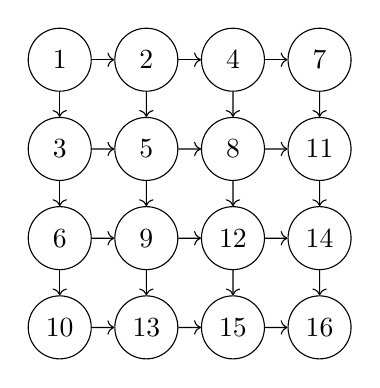
\begin{tikzpicture}[yscale=-1.03,scale=1.1]
	\node [fill=white, draw=black, shape=circle, minimum size=8mm] (1) at (0, 0) {1};
	\node [fill=white, draw=black, shape=circle, minimum size=8mm] (2) at (1, 0) {2};
	\node [fill=white, draw=black, shape=circle, minimum size=8mm] (4) at (2, 0) {4};
	\node [fill=white, draw=black, shape=circle, minimum size=8mm] (7) at (3, 0) {7};
	
	\node [fill=white, draw=black, shape=circle, minimum size=8mm] (3) at (0, 1) {3};
	\node [fill=white, draw=black, shape=circle, minimum size=8mm] (5) at (1, 1) {5};
	\node [fill=white, draw=black, shape=circle, minimum size=8mm] (8) at (2, 1) {8};
	\node [fill=white, draw=black, shape=circle, minimum size=8mm] (11) at (3, 1) {11};
	
	\node [fill=white, draw=black, shape=circle, minimum size=8mm] (6) at (0, 2) {6};
	\node [fill=white, draw=black, shape=circle, minimum size=8mm] (9) at (1, 2) {9};
	\node [fill=white, draw=black, shape=circle, minimum size=8mm] (12) at (2, 2) {12};
	\node [fill=white, draw=black, shape=circle, minimum size=8mm] (14) at (3, 2) {14};
	
	\node [fill=white, draw=black, shape=circle, minimum size=8mm] (10) at (0, 3) {10};
	\node [fill=white, draw=black, shape=circle, minimum size=8mm] (13) at (1, 3) {13};
	\node [fill=white, draw=black, shape=circle, minimum size=8mm] (15) at (2, 3) {15};
	\node [fill=white, draw=black, shape=circle, minimum size=8mm] (16) at (3, 3) {16};
	
	\draw [fill=none, ->] (1) to (3);
	\draw [fill=none, ->] (2) to (5);
	\draw [fill=none, ->] (4) to (8);
	\draw [fill=none, ->] (7) to (11);
	
	\draw [fill=none, ->] (3) to (6);
	\draw [fill=none, ->] (5) to (9);
	\draw [fill=none, ->] (8) to (12);
	\draw [fill=none, ->] (11) to (14);
	
	\draw [fill=none, ->] (6) to (10);
	\draw [fill=none, ->] (9) to (13);
	\draw [fill=none, ->] (12) to (15);
	\draw [fill=none, ->] (14) to (16);
	
	\draw [fill=none, ->] (1) to (2);
	\draw [fill=none, ->] (2) to (4);
	\draw [fill=none, ->] (4) to (7);
	
	\draw [fill=none, ->] (3) to (5);
	\draw [fill=none, ->] (5) to (8);
	\draw [fill=none, ->] (8) to (11);
	
	\draw [fill=none, ->] (6) to (9);
	\draw [fill=none, ->] (9) to (12);
	\draw [fill=none, ->] (12) to (14);
	
	\draw [fill=none, ->] (10) to (13);
	\draw [fill=none, ->] (13) to (15);
	\draw [fill=none, ->] (15) to (16);
\end{tikzpicture}
\caption{An example DAG for a 4x4 pentomino superproblem}\label{fig:dag_example1215}
\end{figure}

For these problems we tested the performance of \dagster\ for different numbers of processor cores, against the  \tinisat\ and \lingeling\ CDCL baselines for different sized problems, the results are shown in figure \ref{fig:performance_graph46461}.
In this figure, we see that \dagster\ is upto an order of magnitude faster (in the median) for these problems than serial sat solvers, but that increasing the number of cores does not necessarily improve performance.
Specifically we suspect that this is because the DAGs of these problems (such as per instance in figure \ref{fig:dag_example1215}) do not support sufficiently many parallel processing streams to take advantage of higher parallel processing cores.

   \begin{figure}[]
        \centering
		\begin{tikzpicture}
		\begin{axis}[
			title={},
			xlabel={$n$},
			ylabel={Execution Time (s)},
			%xmin=0, xmax=0.25,
			%ymin=10.00, ymax=100000.00,
			ymode=log,
			%xtick={0,0.05,0.1,0.15,0.2,0.25},
			%ytick={0,20,40,60,80,100},
			%yticklabel=$\pgfmathprintnumber{\tick}\%$,
			legend pos=south east,
			ymajorgrids=true,
			grid style=dashed,
			xticklabel style={/pgf/number format/fixed},
			width = 350,
			height = 300
		]


\addplot[color=black,line width=0.4pt] coordinates {
(1,2.65920496)(2,13.64072895)(3,33.22629547)(4,87.40588522)(5,184.7756422)(6,344.4516697)(7,522.2698565)(8,973.96888805)(9,1498.1676295)
}node[pos=0.8](endofplotsquare){} ;
\addlegendentry{\tinisat}
\addplot[color=red,line width=0.4pt] coordinates {
(1,2.626594543)(2,17.20426822)(3,62.83456993)(4,151.1784186)(5,288.6084802)(6,430.5156553)(7,612.4651904)(8,892.3813566)(9,1367.4057105)
}node[pos=0.8](endofplotsquare){} ;
\addlegendentry{\lingeling}
\addplot[color=blue!0!green,line width=0.4pt] coordinates {
(1,2.104455948)(2,7.153005123)(3,14.83383656)(4,29.67617917)(5,53.84574914)(6,88.65398169)(7,138.4907691)(8,220.7598681)(9,335.48360325)
}node[pos=0.8](endofplotsquare){} ;
\addlegendentry{\dagster 2 cores}
\addplot[color=blue!15!green,line width=0.4pt] coordinates {
(1,2.117341995)(2,6.11175108)(3,10.45130038)(4,19.09019256)(5,35.06234717)(6,54.44021153)(7,84.62052226)(8,122.59767439999999)(9,187.43380915)
}node[pos=0.8](endofplotsquare){} ;
\addlegendentry{\dagster 3 cores}
\addplot[color=blue!30!green,line width=0.4pt] coordinates {
(1,2.136771917)(2,5.911049366)(3,9.480689049)(4,17.65658808)(5,27.70721459)(6,42.19741297)(7,58.88561153)(8,87.96565247000001)(9,126.90254595)
}node[pos=0.8](endofplotsquare){} ;
\addlegendentry{\dagster 5 cores}
\addplot[color=blue!45!green,line width=0.4pt] coordinates {
(1,2.337931395)(2,5.714944839)(3,9.422580242)(4,17.73626924)(5,28.41895914)(6,42.03511643)(7,56.37598395)(8,80.59561407999999)(9,108.0522034)
}node[pos=0.8](endofplotsquare){} ;
\addlegendentry{\dagster 9 cores}
\addplot[color=blue!60!green,line width=0.4pt] coordinates {
(1,2.414685488)(2,5.935769558)(3,9.943222284)(4,18.572963)(5,29.34904099)(6,43.08808184)(7,57.75251317)(8,82.62288594500001)(9,114.01351985)
}node[pos=0.8](endofplotsquare){} ;
\addlegendentry{\dagster 17 cores}
\addplot[color=blue!75!green,line width=0.4pt] coordinates {
(1,2.553133488)(2,6.305172682)(3,10.45382071)(4,20.15969753)(5,30.57410383)(6,45.34164023)(7,62.43268538)(8,89.43521988500001)(9,125.59903059999999)
}node[pos=0.8](endofplotsquare){} ;
\addlegendentry{\dagster 33 cores}
\addplot[color=blue!90!green,line width=0.4pt] coordinates {
(1,3.191733837)(2,7.478719234)(3,13.02251291)(4,24.2553761)(5,39.13605332)(6,61.48852849)(7,83.68983006)(8,124.21331319999999)(9,149.43823479999998)
}node[pos=0.8](endofplotsquare){} ;
\addlegendentry{\dagster 65 cores}


		\end{axis}
		\end{tikzpicture}
		%\vspace{-18pt}
		\caption[Runtime performance for Pentomino problems]{Runtime performance (specifically medians) of \dagster\ against \tinisat\ and \lingeling\ solvers for different numbers of cores, across $n$, for $n\times n$ grid of $15\times 15$ pentomino problems.}
		\label{fig:performance_graph46461}
    \end{figure}


These Pentomino problems verified the functioning of \dagster\ in providing speedup due to parallelisation in solving larger structured problems with coupled subproblems. 

The invocation to run these experiments is to be found by executed the following command within the code repository:
\begin{verbatim}
~/summer1819/Benchmarks/Pentomino/runme.sh
\end{verbatim}



\clearpage
\section{Counting Models in Parallel - Costas Arrays}

A Costas array is a set of $n$ points in an $nxn$ array such that each column and row contains exactly one point and each of the $n(n-1)/2$ displacement vectors between the the points are distinct; Costas arrays are well known and have various applications, and the process of using search techniques to solve for them is known to be challenging.
Specifically there is an open question about whether any Costas arrays exist notably for sizes 32x32 and 33x33.
Searching processes have revealed that there are none of specific sub-classes of Costas arrays those sizes \cite{748721}, which has invited some to predict that Costas arrays of those sizes exist \cite{conf/ciss/RussoEB10}.
Notwithstanding, searching processes has been conducted at least upto size 29x29 \cite{DBLP:journals/amco/DrakakisIRW11}.


As an example, consider the following 6x6 Costas array in table \ref{table:costas1}:

\begin{table}[h]
\centering
\begin{tabular}{|l|l|l|l|l|l|}
\hline
                         &                          & \cellcolor[HTML]{333333} &                          &                          &                          \\ \hline
                         &                          &                          &                          & \cellcolor[HTML]{333333} &                          \\ \hline
                         &                          &                          &                          &                          & \cellcolor[HTML]{333333} \\ \hline
\cellcolor[HTML]{333333} &                          &                          &                          &                          &                          \\ \hline
                         &                          &                          & \cellcolor[HTML]{333333} &                          &                          \\ \hline
                         & \cellcolor[HTML]{333333} &                          &                          &                          &                          \\ \hline
\end{tabular}
\caption{An example 6x6 Costas array}\label{table:costas1}
\end{table}
from this example Costas array we can see that there is exactly one filled-in cell for every column and row; additionally we can see that the vector displacement between any of the filled-in cells is unique and that there are no two sets of cells that have the same spacing between them. Particularly if we we tabulate all of the $n(n-1)/2$ displacements between pairs of nodes in table \ref{table:costas2} we can see that all the displacements values along each of the rows are unique.

\begin{table}[h]
\centering
\begin{tabular}{l|l|llll}
\cline{2-6}
                                 & \textbf{1} & \multicolumn{1}{l|}{\textbf{2}} & \multicolumn{1}{l|}{\textbf{3}} & \multicolumn{1}{l|}{\textbf{4}} & \multicolumn{1}{l|}{\textbf{5}} \\ \hline
\multicolumn{1}{|l|}{\textbf{1}} & +2         & \multicolumn{1}{l|}{-5}         & \multicolumn{1}{l|}{+4}         & \multicolumn{1}{l|}{-3}         & \multicolumn{1}{l|}{+1}         \\ \hline
\multicolumn{1}{|l|}{\textbf{2}} & -3         & \multicolumn{1}{l|}{-1}         & \multicolumn{1}{l|}{+1}         & \multicolumn{1}{l|}{-2}         &                                 \\ \cline{1-5}
\multicolumn{1}{|l|}{\textbf{3}} & +1         & \multicolumn{1}{l|}{-4}         & \multicolumn{1}{l|}{+2}         &                                 &                                 \\ \cline{1-4}
\multicolumn{1}{|l|}{\textbf{4}} & -2         & \multicolumn{1}{l|}{-3}         &                                 &                                 &                                 \\ \cline{1-3}
\multicolumn{1}{|l|}{\textbf{5}} & -1         &                                 &                                 &                                 &                                 \\ \cline{1-2}
\end{tabular}
\caption{The displacements of the example 6x6 Costas array \ref{table:costas1}, organised by horisontal distance in rows, by horisontal offset in columns}\label{table:costas2}
\end{table}

Costas arrays are known to exist for many sizes, and for every Costas array, there are potentially 8 symmetry mappings of the same array that are also Costas arrays (by rotations and flip, ie. the dihedral group), consider numbers of Costas arrays by size given by online encyclopedia of integer sequences (OEIS): \url{https://oeis.org/A008404} and \url{https://oeis.org/A001441}.

The investigative question therefore is: if we can encode the Costas problem into SAT, and then decompose the resulting SAT problem for accelerated solving using \dagster.
Particularly the SAT encoding of the Costas problem was produced with optional symmetry breaking constraints to break dihedral mappings, particularly with lex-leader symmetry breaking, and a more simplified and less total symmetry breaking as found in \cite{conf/ciss/RussoEB10}.
From this SAT problem we considered primarily two different ways of decomposing the SAT problem.
\begin{enumerate}
\item	Inspired by the construction of such tables as table \ref{table:costas2}, we considered a decomposition of iteratively constructing Costas arrays from the bottom of the table up. This decomposition proved to be poor performing as a combinatorial number of intermediate solutions between depths were created
\item	Taking a much simpler approach of decomposing the problem into two parts, the first being placing the first two columns of the Costas array, and the second part of the problem being that the rest of the Costas array would be filled in. This proved to be more effective decomposition of the problem. See Figure \ref{fig:dag_example121}.
\end{enumerate}

\begin{figure}[h]
\centering
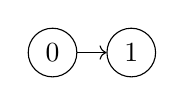
\begin{tikzpicture}
	\node [fill=white, draw=black, shape=circle] (0) at (0, 0) {0};
	\node [fill=white, draw=black, shape=circle] (1) at (1, 0) {1};
	\draw [fill=none, ->] (0) to (1);
\end{tikzpicture}
\caption{A simplified DAG structure for the Costas decomposition}\label{fig:dag_example121}
\end{figure}

The performance of \dagster\ at solving Costas problems for different sized Costas arrays is given in Figure \ref{fig:performance_graph3}.
In this figure the time taken to count all the Costas arrays of a given size is plotted against the size of the problem for different numbers of cores against the time taken to do the same thing running the serial baseline CDCL procedure implemented in \tinisat\ (shown in black).
From this figure we can see that for larger sized Costas arrays that \dagster\ shows significantly improved performance in solving the Costas model counting problem, where the performance increases with the number of cores.
However it is also noticed that for smaller and easier Costas problems (of size $nxn$ where $n<10$) that the parallel overhead of using \dagster\ is the primary determinant of the solution time, where the greater the number of cores the larger the overhead and the slower the process.

With this simulation we can verify that \dagster\ can be used to speedup solving performance on the types of problems which are geometrically difficult and resemble research-interesting questions.

The Costas simulation that produced the data shown in Figure \ref{fig:performance_graph3} can be invoked from the \dagster\ repository by executing:
\begin{verbatim}
/summer1819/Benchmarks/run.sh
\end{verbatim}
Where the script compiles and invokes the `generate-costas-N' program from inside that same directory.

   \begin{figure}[h]
        \centering
		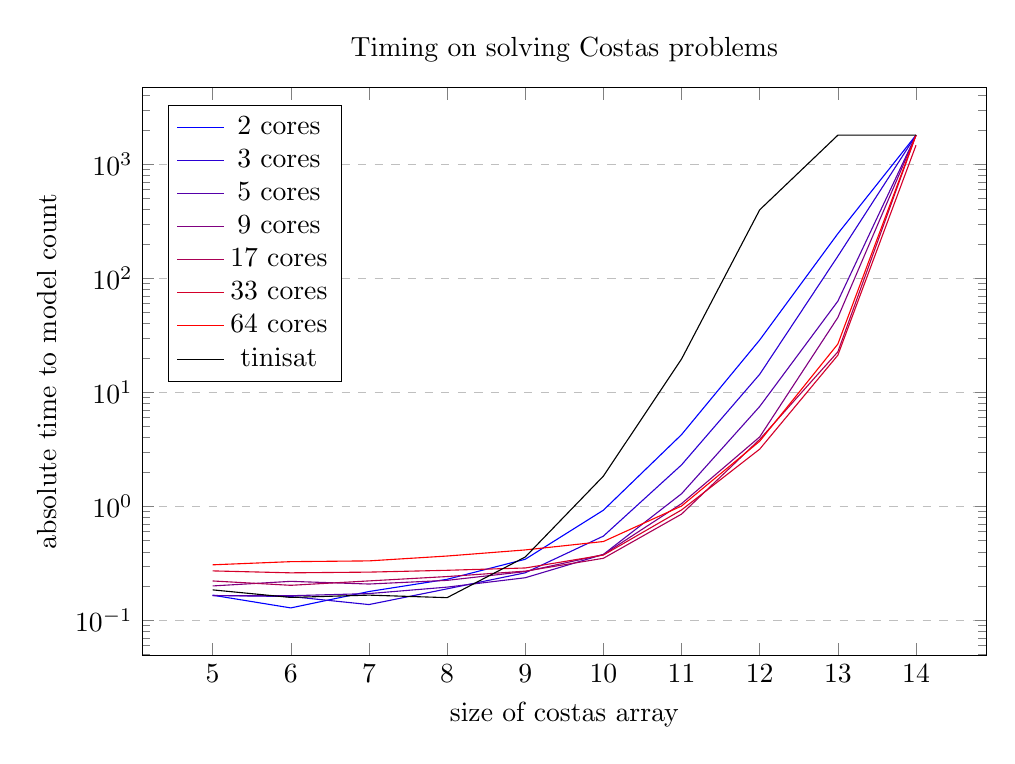
\begin{tikzpicture}
		\begin{axis}[
			title={Timing on solving Costas problems},
			xlabel={size of costas array},
			ylabel={absolute time to model count},
			%xmin=0, xmax=0.25,
			%ymin=10.00, ymax=100000.00,
			ymode=log,
			%xmode=log,
			%xtick={0,0.05,0.1,0.15,0.2,0.25},
			%ytick={0,20,40,60,80,100},
			%yticklabel=$\pgfmathprintnumber{\tick}\%$,
			legend pos=north west,
			ymajorgrids=true,
			grid style=dashed,
			xticklabel style={/pgf/number format/fixed},
			width = 350,
			height = 250
		]






\addplot[color=red!0.0!blue,line width=0.4pt] coordinates {
(5,0.16651105880737305)(6,0.128767728805542)(7,0.17928266525268555)(8,0.229478120803833)(9,0.3440828323364258)(10,0.9262895584106445)(11,4.26284122467041)(12,28.817259788513184)(13,246.72397589683533)(14,1801.013244152069)
}node[pos=0.8](endofplotsquare){} ;
\addlegendentry{2 cores}
\addplot[color=red!16.666666666666668!blue,line width=0.4pt] coordinates {
(5,0.16553544998168945)(6,0.16209650039672852)(7,0.1377730369567871)(8,0.18923521041870117)(9,0.2616755962371826)(10,0.5489482879638672)(11,2.313494920730591)(12,14.413764238357544)(13,156.3844666481018)(14,1801.0142397880554)
}node[pos=0.8](endofplotsquare){} ;
\addlegendentry{3 cores}
\addplot[color=red!33.333333333333336!blue,line width=0.4pt] coordinates {
(5,0.164872407913208)(6,0.16470789909362793)(7,0.17198729515075684)(8,0.19599699974060059)(9,0.23682069778442383)(10,0.3795149326324463)(11,1.291374921798706)(12,7.523766040802002)(13,63.10072612762451)(14,1801.0149838924408)
}node[pos=0.8](endofplotsquare){} ;
\addlegendentry{5 cores}
\addplot[color=red!50.0!blue,line width=0.4pt] coordinates {
(5,0.20067811012268066)(6,0.22022223472595215)(7,0.20856070518493652)(8,0.22462010383605957)(9,0.2682313919067383)(10,0.37816452980041504)(11,1.0574686527252197)(12,4.069439888000488)(13,45.39408540725708)(14,1801.0188295841217)
}node[pos=0.8](endofplotsquare){} ;
\addlegendentry{9 cores}
\addplot[color=red!66.66666666666667!blue,line width=0.4pt] coordinates {
(5,0.22196483612060547)(6,0.2032465934753418)(7,0.22217583656311035)(8,0.24254584312438965)(9,0.2705719470977783)(10,0.35074734687805176)(11,0.8557615280151367)(12,3.8713788986206055)(13,22.67898917198181)(14,1801.0271427631378)
}node[pos=0.8](endofplotsquare){} ;
\addlegendentry{17 cores}
\addplot[color=red!83.33333333333333!blue,line width=0.4pt] coordinates {
(5,0.2719554901123047)(6,0.2614936828613281)(7,0.2652904987335205)(8,0.27526402473449707)(9,0.28845834732055664)(10,0.37433934211730957)(11,0.9312081336975098)(12,3.1793856620788574)(13,21.185994863510132)(14,1469.3303191661835)
}node[pos=0.8](endofplotsquare){} ;
\addlegendentry{33 cores}
\addplot[color=red!100.0!blue,line width=0.4pt] coordinates {
(5,0.3074929714202881)(6,0.32775092124938965)(7,0.33288002014160156)(8,0.36718130111694336)(9,0.415346622467041)(10,0.4921422004699707)(11,1.0077219009399414)(12,3.730285882949829)(13,26.540127277374268)(14,1802.017567873001)
}node[pos=0.8](endofplotsquare){} ;
\addlegendentry{64 cores}
\addplot[color=black,line width=0.4pt] coordinates {
(5,0.18535566329956055)(6,0.15912103652954102)(7,0.16672492027282715)(8,0.15842223167419434)(9,0.36010169982910156)(10,1.843733787536621)(11,19.61815071105957)(12,398.9100785255432)(13,1801.0124578475952)(14,1801.01256108284)
}node[pos=0.8](endofplotsquare){} ;
\addlegendentry{tinisat}

		\end{axis}
		\end{tikzpicture}
		%\vspace{-18pt}
		\caption[Runtime to solve Costas arrays]{Runtime to solve Costas arrays, by core count and costas array size w/ 1800s timeout}
		\label{fig:performance_graph3}
    \end{figure}





\clearpage
\section{Accelerating Unsatisfiability Proofs via Parallelisation}

Empirical studies of the Boolean satisfiability problem late last century identified and studied a notion of empirically {\em hard} problems.
The earliest works studied formulae occurring in conjunctive normal form with all disjunctive clauses having a fixed length $k$.
A range of studies of this ``{\em $k$-Satisfiability}'' problem have been undertaken treating different values of $k$, and other more flexible concepts of structural invariants.
Taking $k=3$ and studying sets of pseudo-random problems researchers found that so-called ``hard'' problems occur when the ratio of the count of clauses to the count of problem variables is approximately $4.26$~\cite{cheeseman:etal:1991}. 
Here we present a small study of pseudo-random $3$-Satisfiability using the problem distributions associated with Dubois et al. (2000)\cite{dubois:etal:2000}.

Somewhat trivially---i.e. primarily due to a portfolio effect---the hybrid search implemented in \dagster\ outperforms CDCL baselines in hard satisfiable random instances.
For satisfiable $3$-Satisfiability the best solution procedure is a local search~\cite{pham:etal:2008}. 
Our hybrid configuration of  \dagster\ allows any number of such searches to be scheduled to run more-or-less independently in parallel on your cluster.
Thus, not only is this parallel system better than CDCL here, courtesy of implementing a local search, it is also faster than running a serial local search procedure, because the expected walltime to a solution being emitted is at the lower end of the runtime distribution of that stochastic procedure.
Here, we focus on the more interesting setting, accelerating search in a family of unsatisfiable $3$-Satisfiability problems.

In our first result, we accelerate the walltime performance of the default implementation of CDCL in \tinisat, by leveraging the hybrid search mode, using the local search to generate a complete set of relatively easy UNSAT subproblems that can be solved independently in parallel.
A comparison of runtime of \dagster\ as compared with the serial CDCL procedure in \tinisat\ is given in Figure~\ref{fig:3UNSAT_140random}. 
Specifically, we can decompose the problem using a 2 node DAG in which the ``source'' node indexes $94\%$ of clauses, and this communicates solutions to a ``sink'' node that includes all the clauses from the concrete problem at hand.
What is communicated is a small prefix of the total subproblem valuation. 
The problem at the source node, with only  $94\%$ of clauses, is easily satisfiable using a local search, and indeed the hybrid procedure can quickly enumerate all solutions to that subproblem and subsequently the CDCL procedure can prove that no further solutions exists.
The problem of proving that the concrete problem in unsatisfiable, for each of the valuations associated with the source node subproblem, is extremely easy.

%\begin{figure}
  \centering
  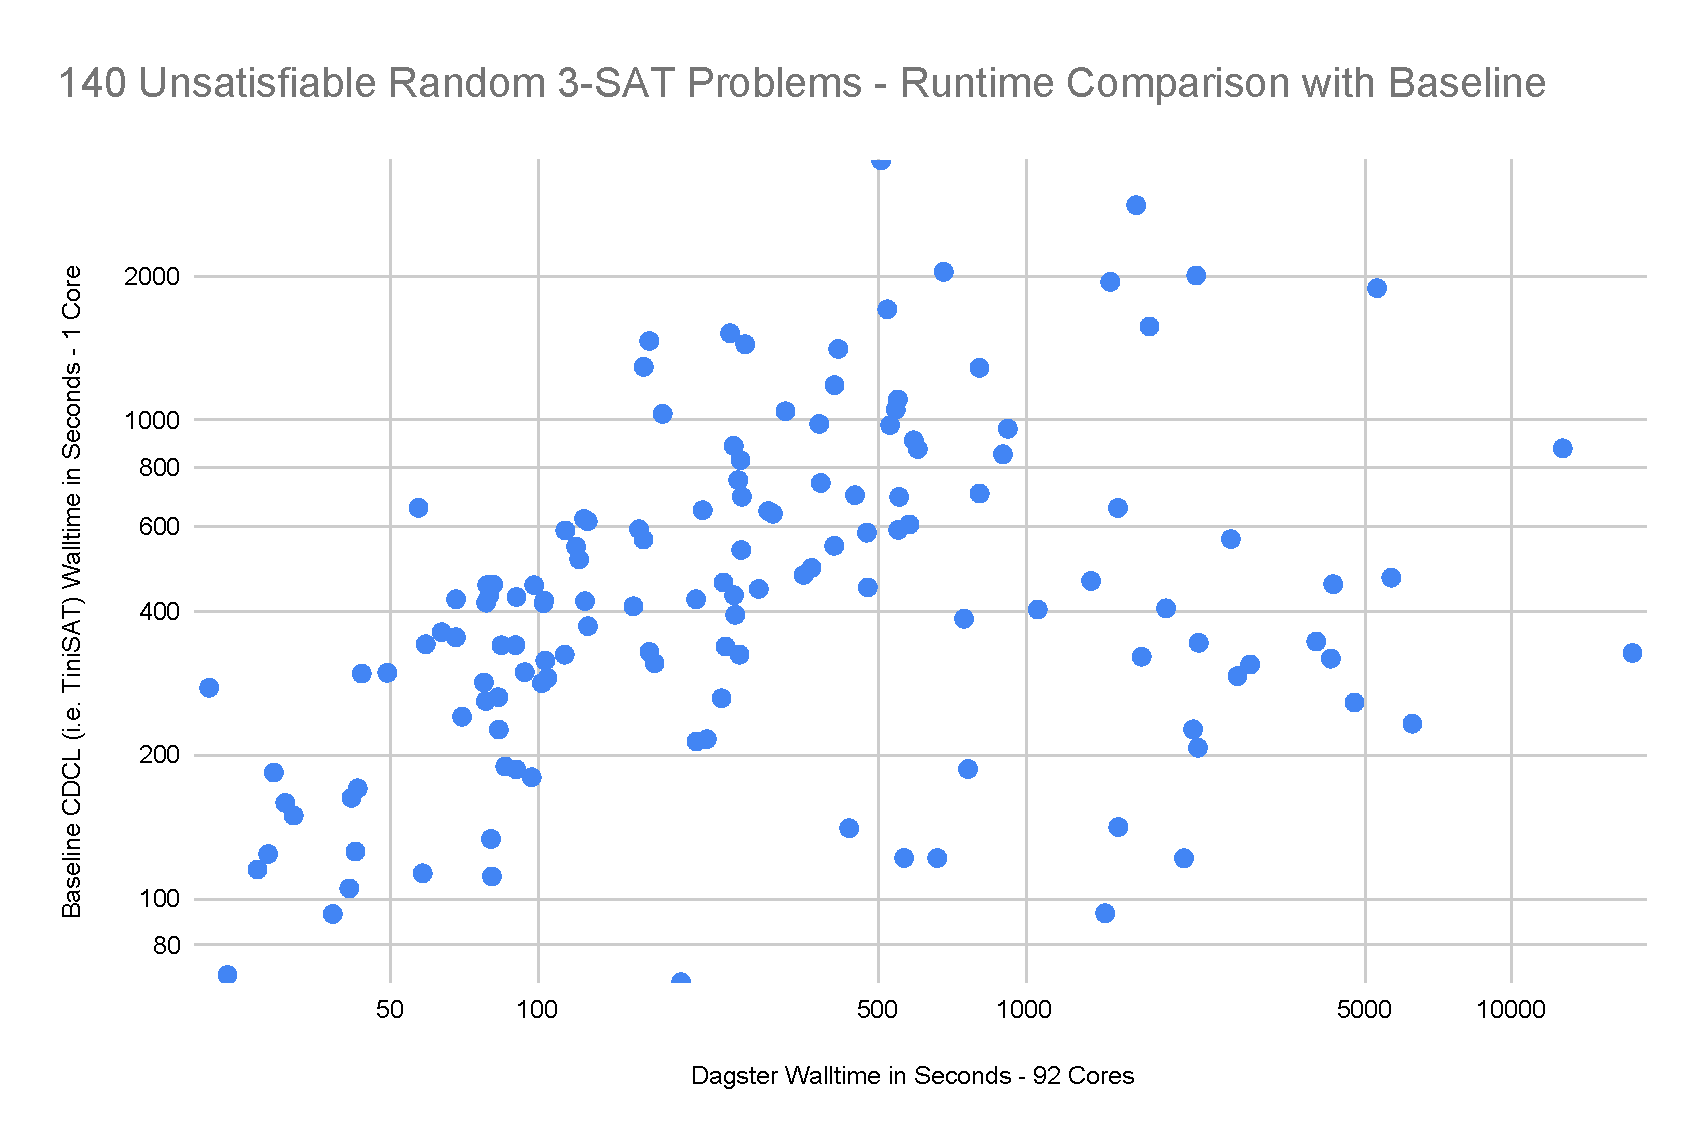
\includegraphics[width=.8\columnwidth]{./figs/3UNSAT_140random.pdf}
  \caption[Scatterplot of Tinisat against Dagster for random unsatisfiable 3Sat instances]{Logscale scatter plot of runtime distributions of \mbox{TiniSAT} (vertical) and  \mbox{Dagster} using 92 cores (horizontal) on pseudo-random unsatisfiable $3$-Satisfiability problem instances.\label{fig:3UNSAT_140random}}
\end{figure}


   \begin{figure}[]
        \centering
		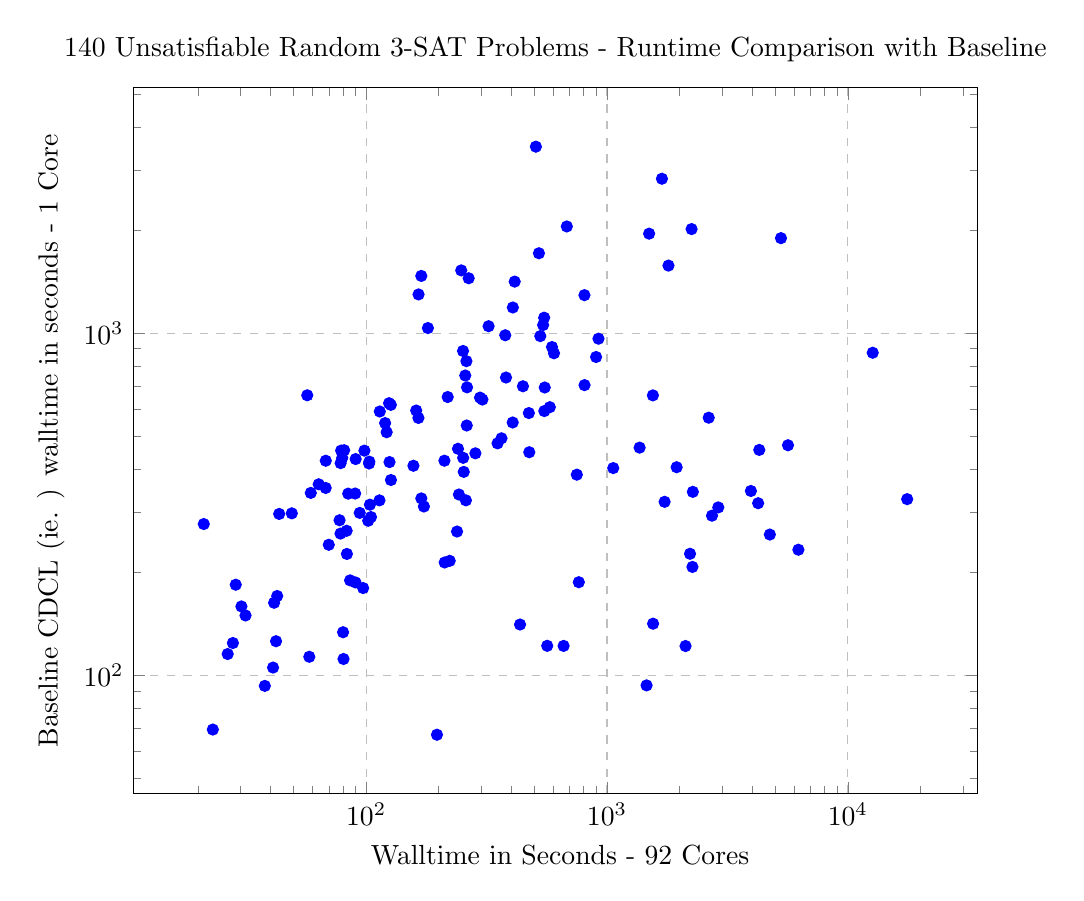
\begin{tikzpicture}
		\begin{axis}[
			title={140 Unsatisfiable Random 3-SAT Problems - Runtime Comparison with Baseline},
			xlabel={\dagster\ Walltime in Seconds - 92 Cores},
			ylabel={Baseline CDCL (ie. \tinisat) walltime in seconds - 1 Core},
			%xmin=0, xmax=0.25,
			%ymin=10.00, ymax=100000.00,
			ymode=log,
			xmode=log,
			%xtick={0,0.05,0.1,0.15,0.2,0.25},
			%ytick={0,20,40,60,80,100},
			%yticklabel=$\pgfmathprintnumber{\tick}\%$,
			legend pos=south east,
			ymajorgrids=true,
			xmajorgrids=true,
			grid style=dashed,
			xticklabel style={/pgf/number format/fixed},
			width = 350,
			height = 300
		]


\addplot[color=blue,only marks] coordinates {
(42.26,125.745)(119.867,545.704)(2728.217,292.677)(67.931,352.727)(21.179,276.65)(322.382,1047.232)(240.595,459.067)(78.358,416.759)(660.406,121.842)(1550.594,657.514)(43.543,296.155)(261.625,536.902)(80.2,133.574)(506.602,3505.237)(121.648,513.245)(1061.421,403.139)(97.171,179.823)(41.486,162.886)(126.765,372.093)(806,1290.684)(4240.705,318.299)(2643.525,565.834)(590.973,910.356)(351.253,476.16)(84.247,339.432)(447.676,699.161)(763.726,187.065)(113.936,589.902)(77.559,283.815)(180.447,1034.351)(1690.419,2824.716)(49.133,297.309)(27.976,124.23)(1553.507,141.486)(101.967,282.867)(1495.695,1952.363)(104.73,289.984)(2896.473,309.438)(406.422,1187.694)(126.619,616.863)(102.826,415.73)(266.463,1446.01)(549.248,591.68)(211.846,213.583)(23.089,69.41)(124.491,623.812)(90.453,428.356)(248.186,1524.726)(921.673,962.741)(26.615,115.363)(173.687,311.332)(1459.816,93.42)(1799.701,1574.52)(521.555,1711.07)(80.547,111.57)(254.275,393.006)(564.572,121.919)(196.821,67.018)(475.597,448.536)(169.425,1468.822)(380.813,741.443)(1365.755,462.605)(30.35,158.917)(2244.52,2013.101)(364.733,492.594)(2262.841,207.311)(1734.328,321.255)(435.473,140.696)(81.024,454.584)(79.552,431.68)(548.294,1108.946)(378.084,985.383)(602.305,872.929)(222.258,215.967)(37.967,93.092)(4742.795,257.769)(262.324,694.06)(58.079,113.235)(6232.027,232.727)(242.733,337.452)(1946.22,405.46)(260.738,827.722)(169.469,328.716)(113.582,324.442)(749.381,385.727)(164.833,564.966)(5641.305,470.067)(528.534,979.646)(78.755,453.489)(103.65,315.154)(28.745,183.927)(2118.508,121.737)(161.348,593.823)(58.911,341.096)(63.529,361.476)(3958.052,345.572)(82.985,264.38)(542.899,1055.738)(257.885,751.644)(90.344,186.763)(2271.456,343.524)(157.159,409.5)(42.722,170.464)(252.424,886.519)(98.35,453.322)(165.033,1296.811)(297.089,647.719)(78.255,259.416)(56.956,657.919)(303.857,639.407)(2211.474,226.46)(551.438,693.299)(5275.306,1894.192)(218.042,650.364)(413.741,1413.715)(41.065,105.315)(259.474,324.486)(238.411,263.036)(405.909,547.863)(900.781,851.23)(125.022,419.773)(67.987,423.571)(806.681,704.496)(680.987,2048.929)(90.016,339.74)(94.047,298.174)(12679.367,875.948)(83.19,226.217)(4287.566,455.582)(85.779,189.365)(103.114,420.958)(252.831,431.952)(17628.641,327.106)(31.568,149.551)(69.96,240.616)(284.138,445.204)(578.942,607.365)(473.695,583.777)(211.334,423.656)
}node[pos=0.8](endofplotsquare){} ;


		\end{axis}
		\end{tikzpicture}
		%\vspace{-18pt}
  \caption{Logscale scatter plot of runtime distributions of \tinisat\ (vertical) and \dagster\ using 92 cores (horizontal) on pseudo-random unsatisfiable $3$-Satisfiability problem instances.\label{fig:3UNSAT_140random}}
    \end{figure}


In conclusion, our hybrid solver can, by virtue of local search, easily enumerate the solutions to an underconstrained subproblem, and by virtual of parallelism quickly eliminate those solution candidates using systematic search. 

\clearpage
\section{Decomposing Software Verification Problems for Use in \dagster}

Software verification problems are extremely important and finding a way to decompose them is critical to making proper use of \dagster. We will consider one pipeline that produces SAT problems from C and C++ source code and a preliminary approach which results in a working decomposition for \dagster.

We use the tool CBMC, which is a bounded model checker for C and C++ programs, to generate the SAT problems. CBMC takes a program, which we want to verify certain properties about, and broadly speaking it passes it through 3 stages to result in the SAT formula. We will work through the example code in Figure \ref{ex1_code} to illustrate the process\footnote{CBMC can perform other safety checks in relation to memory and array bounds etc.. Our example will only consider an assertion that the user wants to be satisfied.}.
\begin{enumerate}
    \item In the first stage the given C/C++ program is converted into a GOTO program, which results in all code that performs a jump of some kind such as if statements, jumps and loops being converted into an equivalent goto statement which optionally has a guard or condition attached to it. The resulting GOTO program will only contain guarded goto statements\footnote{Which can be thought of, and are represented as, a conditional "if !X THEN GOTO Y".}, assignments, assertions, labels and goto instructions.
    \item In the second stage the GOTO program is converted into single static assignment (SSA) form as CBMC performs loop unwinding which is done to a fixed bound\footnote{The unwinding can be determined manually by the user or left to the program to verify when enough unwinding has been done. We will not go into the details of this here.}. In SSA form variables can only be assigned once and with a special $\phi$ function are inserted at merge points to determine which of the possible instances of the variable are now being referred to. An example of this conversion can be seen in Figure \ref{ex1_ssa}, where $\phi$ nodes have been expanded into a form that uses the C ternary operator "?:".
    \item In the final stage the SSA form is converted into a formula, by turning the assignments into equalities and forming the conjunction of all them as in Figure \ref{ex1_formula}, noting that the property to be checked is negated which in this case means we check to see if crash\_5 $= 1$. This formula is then converted into a form amenable for SAT by a process known as bit-blasting, we will not go into the details of that here.
\end{enumerate}

\begin{figure}[h]
  \centering
  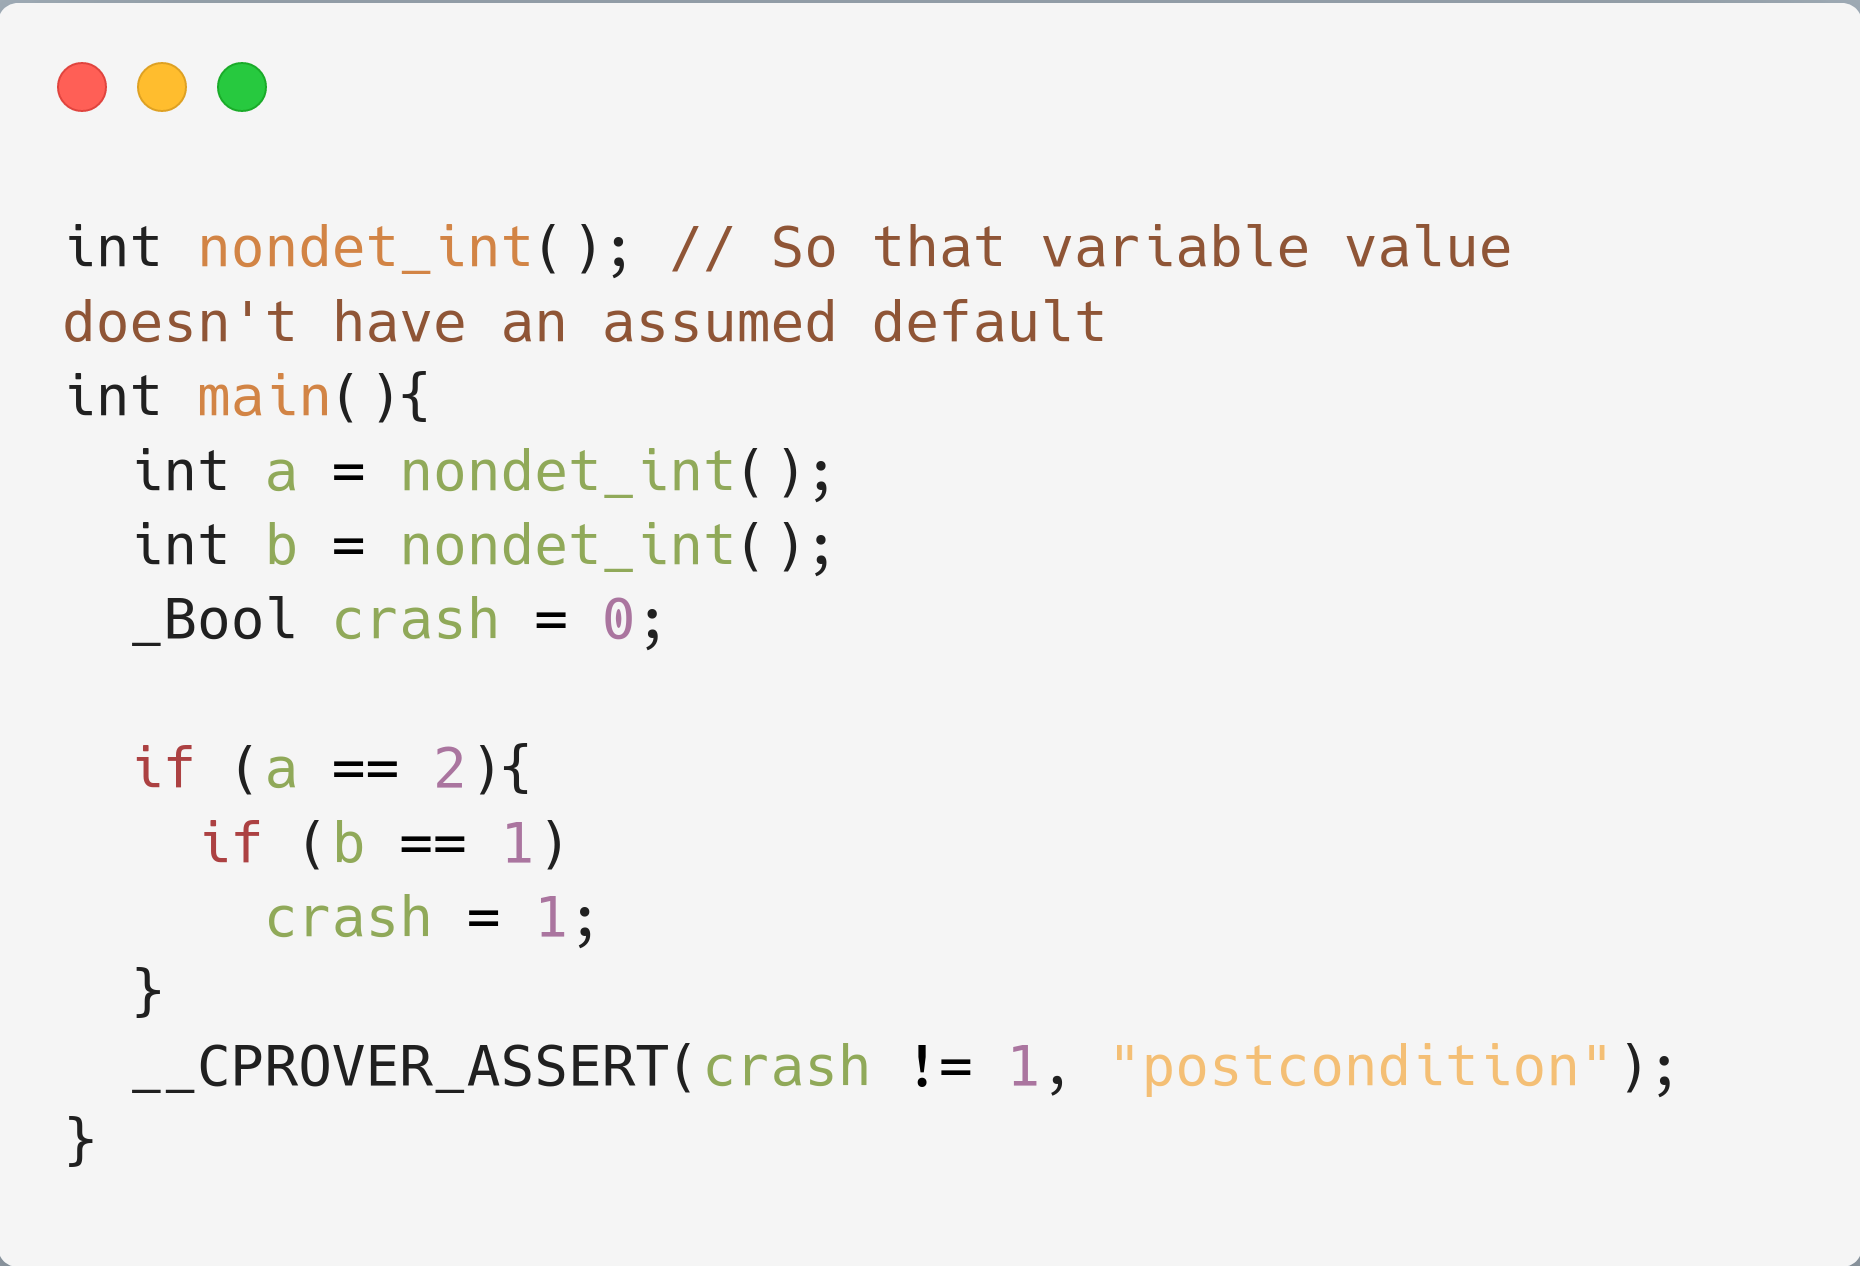
\includegraphics[width=6cm]{./figs/ex1_code.png}
  \caption{Example code in C.}
  \label{ex1_code}
\end{figure}
\begin{figure}[h]
  \centering
  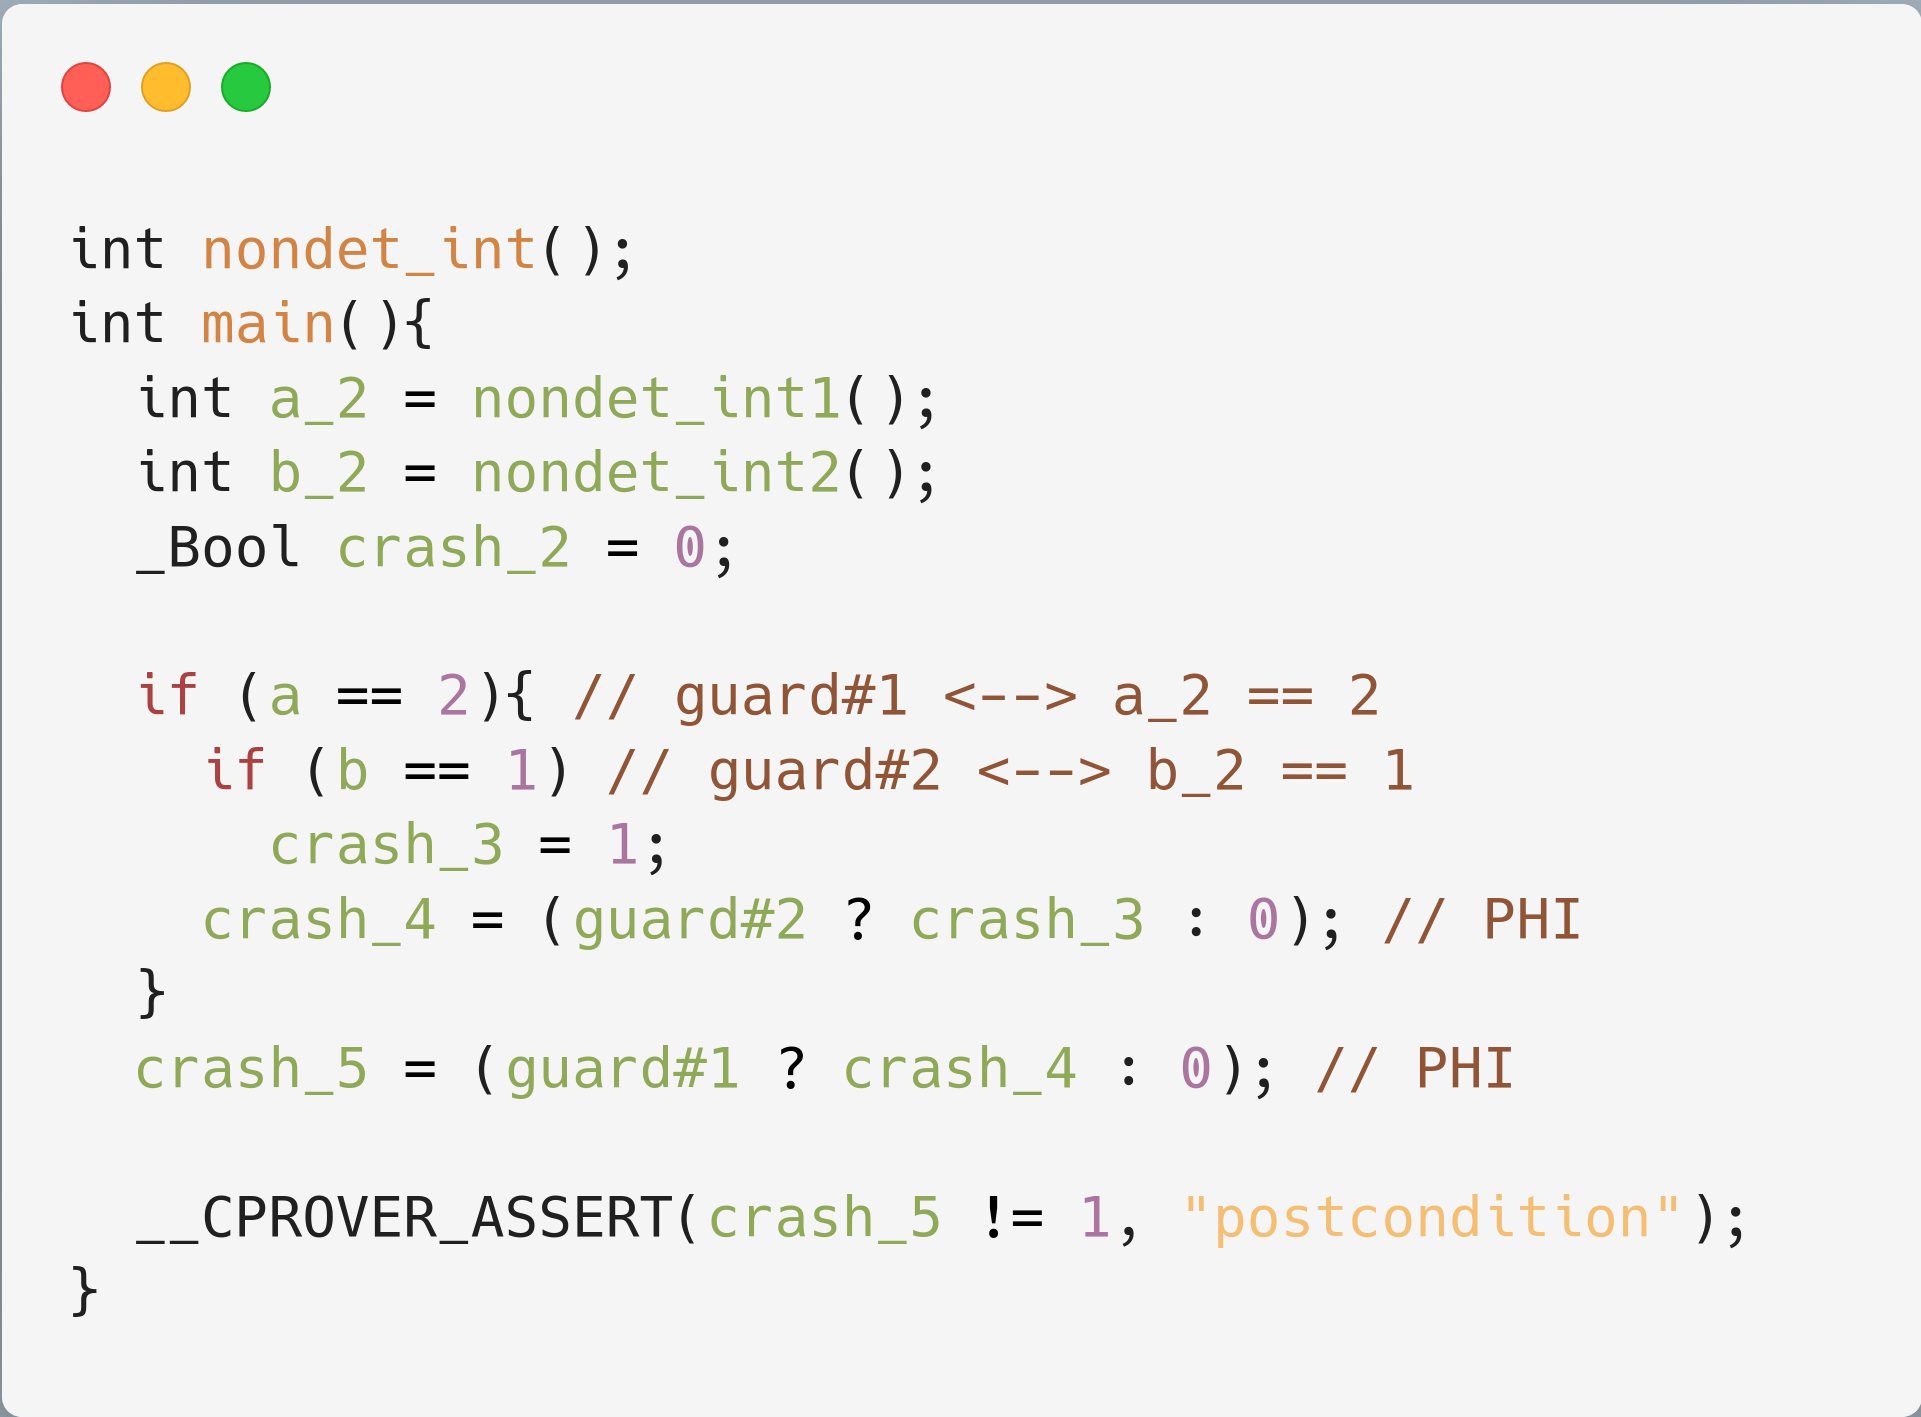
\includegraphics[width=6cm]{./figs/ex1_ssa.png}
  \caption{Conversion of code into SSA form.}
  \label{ex1_ssa}
\end{figure}
\begin{figure}[h]
  \centering
  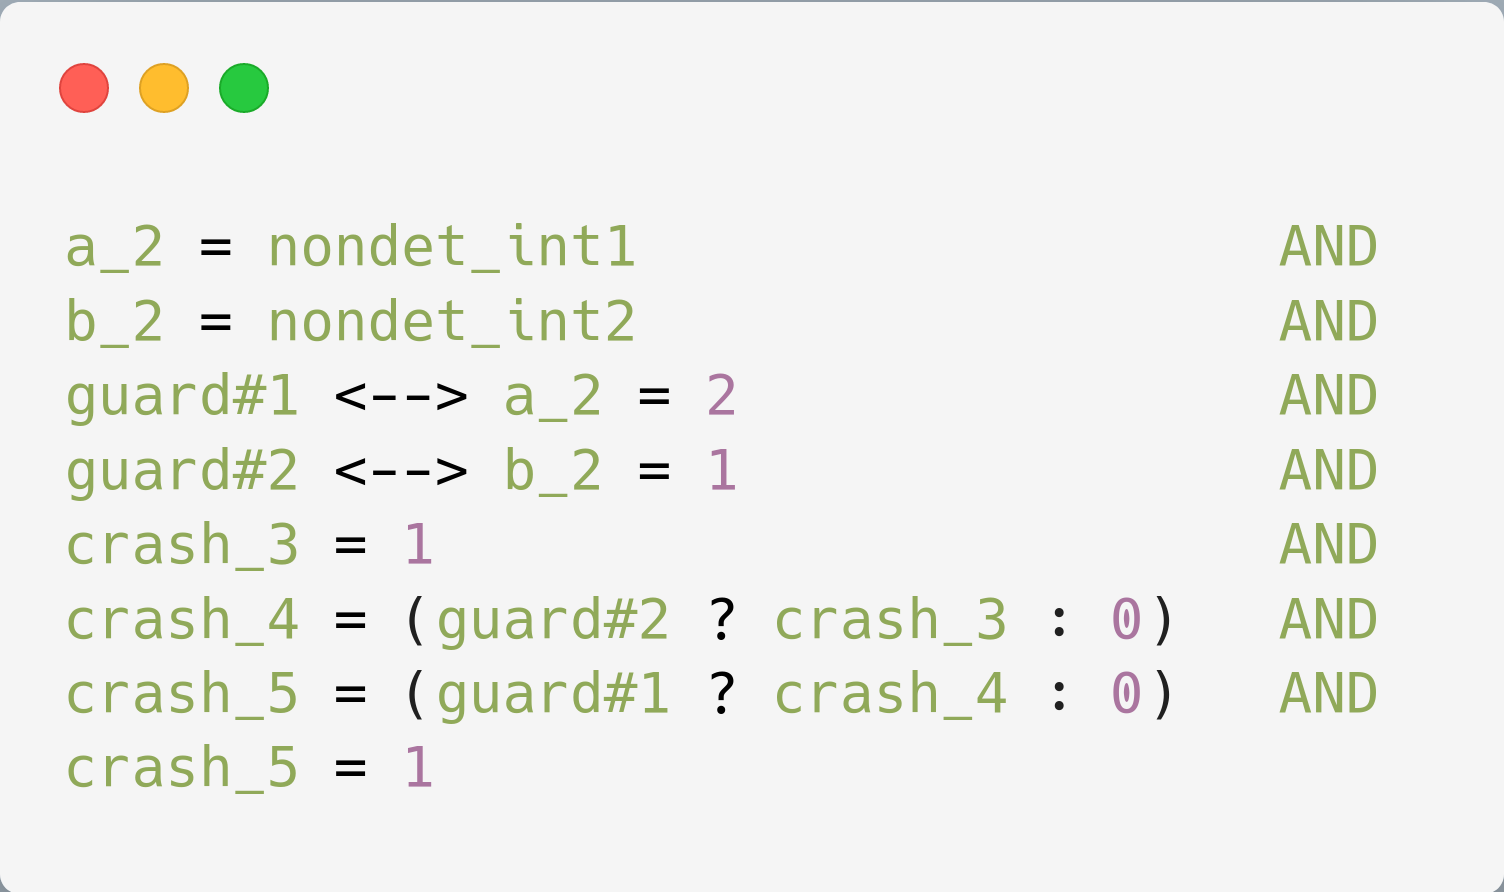
\includegraphics[width=6cm]{./figs/ex1_formula.png}
  \caption{Resultant formula from conversion.}
  \label{ex1_formula}
\end{figure}

We are able to produce a decomposition for this program by considering the formula as it is represented in SSA form. The resulting decomposition that we create will have four nodes, see Figure \ref{ex1_dag}. The first node contains clauses that relate to calculating the goal and determining the values that guard\#1 and guard\#2 should be to reach that goal. These guard values will be communicated to nodes two and three which contain clauses that calculate the corresponding the values for $a$ and $b$ separately as the variable values are independent of one another. The final node will merge the results of nodes two and three and confirm that they cohere to form a solution.



\begin{figure}[h]
\centering
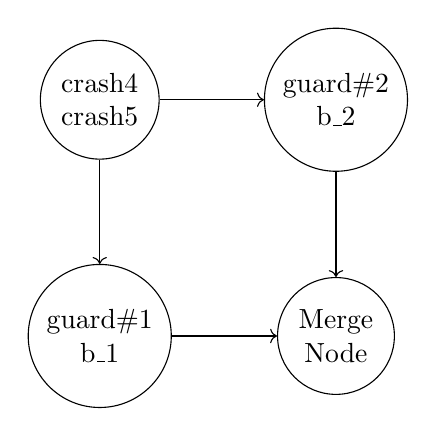
\begin{tikzpicture}
	\node [fill=white, draw=black, shape=circle,align=center] (0) at (0, 3) {crash4\\ crash5};
	\node [fill=white, draw=black, shape=circle,align=center] (1) at (3, 3) {guard$\#$2\\ b\_2};
	\node [fill=white, draw=black, shape=circle,align=center] (2) at (0, 0) {guard$\#$1\\ b\_1};
	\node [fill=white, draw=black, shape=circle,align=center] (3) at (3, 0) {Merge\\Node};
	\draw [fill=none, ->] (0) to (1);
	\draw [fill=none, ->] (0) to (2);
	\draw [fill=none, ->] (1) to (3);
	\draw [fill=none, ->] (2) to (3);
\end{tikzpicture}
  \caption{DAG for example code.}
  \label{ex1_dag}
\end{figure}


Using a similar method we can produce a decomposition for a program with three independent conditionals \ref{ex2_code}, which will result in three completely independent sub-problems that are embarrassingly parallel \ref{ex2_dag}.

\begin{figure}
    \centering
    \begin{minipage}{0.45\textwidth}
        \centering

  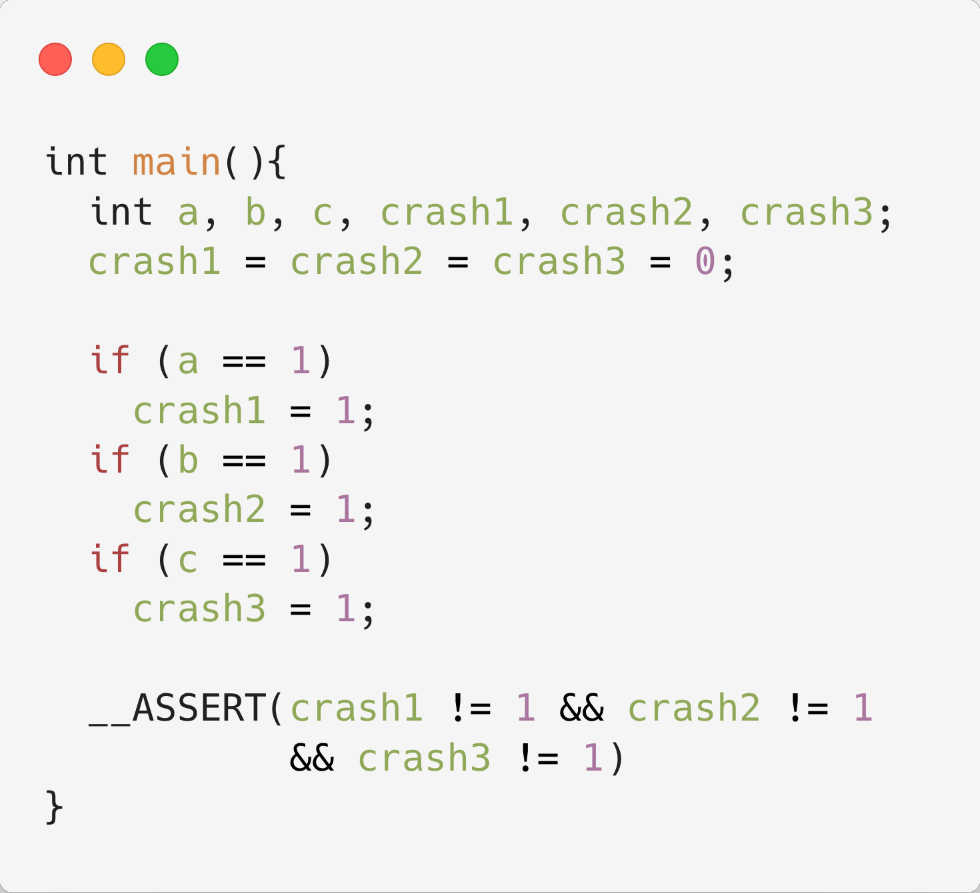
\includegraphics[width=6cm]{./figs/ex2_code.png}
  \caption{Three independent conditionals.}
  \label{ex2_code}

    \end{minipage}\hfill
    \begin{minipage}{0.45\textwidth}
        \centering

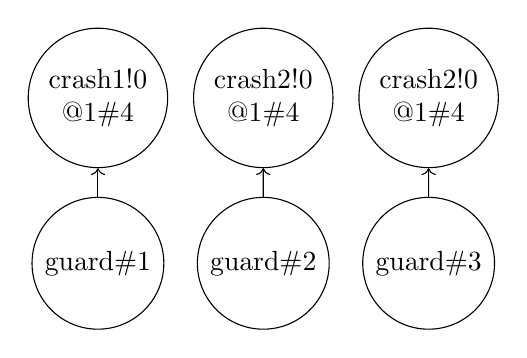
\begin{tikzpicture}[scale=0.7]
	\node [fill=white, draw=black, shape=circle,align=center] (0) at (0, 0) {guard$\#$1};
	\node [fill=white, draw=black, shape=circle,align=center] (1) at (0, 3) {crash1!0\\@1$\#$4};
	\node [fill=white, draw=black, shape=circle,align=center] (2) at (3, 0) {guard$\#$2};
	\node [fill=white, draw=black, shape=circle,align=center] (3) at (3, 3) {crash2!0\\@1$\#$4};
	\node [fill=white, draw=black, shape=circle,align=center] (4) at (6, 0) {guard$\#$3};
	\node [fill=white, draw=black, shape=circle,align=center] (5) at (6, 3) {crash2!0\\@1$\#$4};
	\draw [fill=none, ->] (0) to (1);
	\draw [fill=none, ->] (2) to (3);
	\draw [fill=none, ->] (4) to (5);
\end{tikzpicture}
  \caption{DAG for the problem with three independent conditionals.}
  \label{ex2_dag}


    \end{minipage}
\end{figure}



Finally, we are also able to decompose software verification problems which contain loops where variables are independently acted upon \ref{ex3_code}. This will result in the first node computing the goal as before, and then two child nodes which deal with calculating the resultant values for the independent variables $a$ and $b$, whose results are then passed onto the merge node cf. \ref{ex3_dag}. 


\begin{figure}
    \centering
    \begin{minipage}{0.45\textwidth}
        \centering

  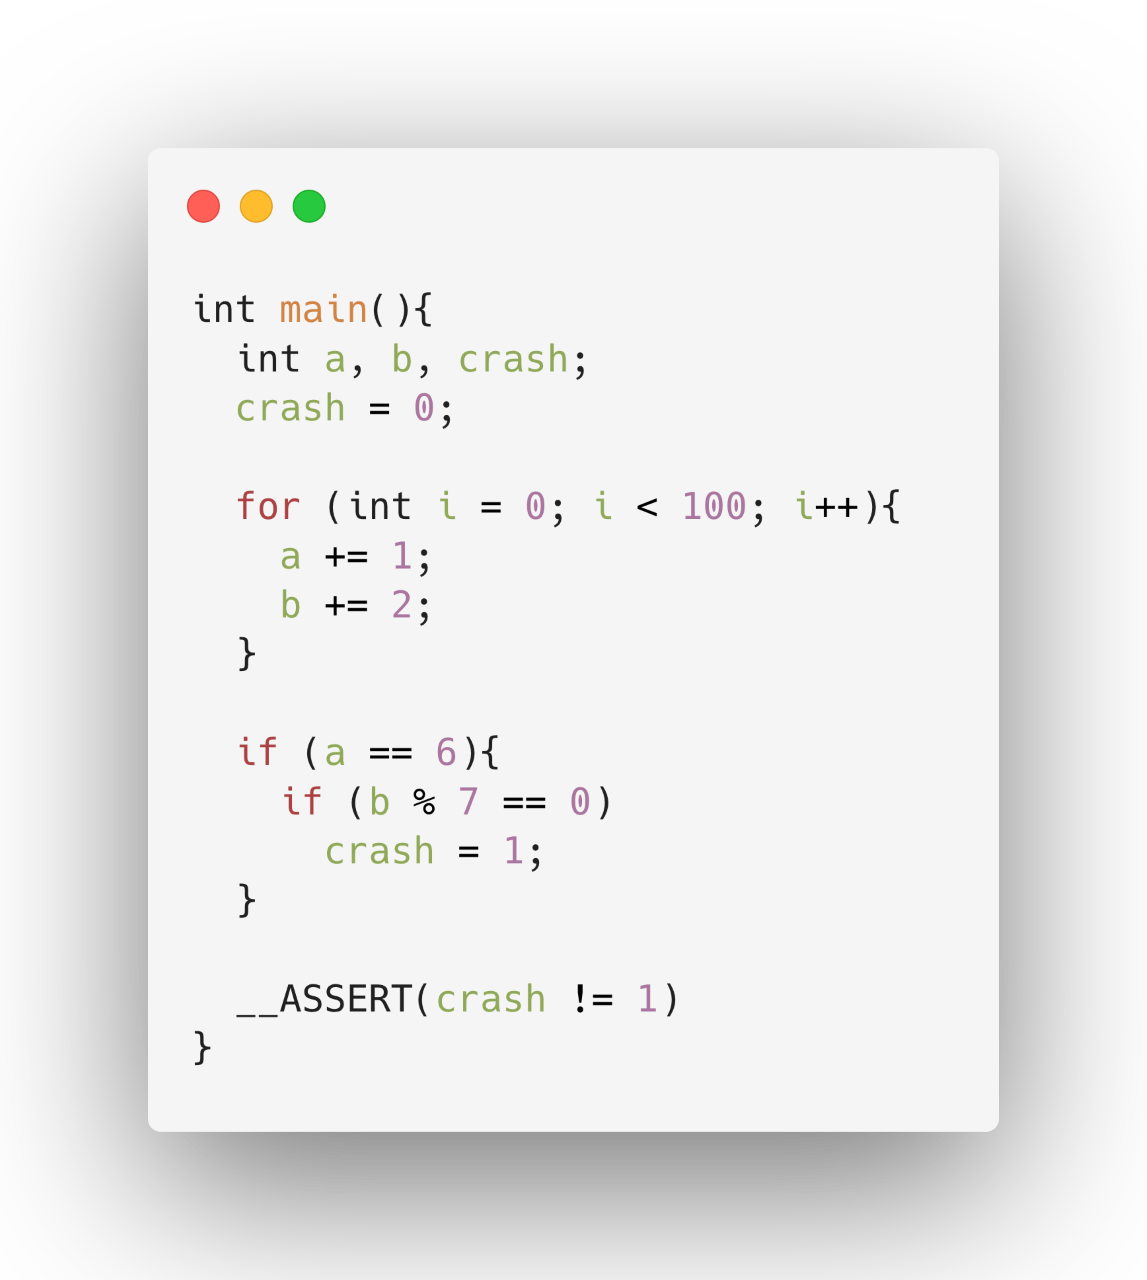
\includegraphics[width=6cm]{./figs/ex3_code.png}
  \caption{A crash is triggered based on the resulting values of two variables acted upon independently in a loop.}
  \label{ex3_code}


    \end{minipage}\hfill
    \begin{minipage}{0.45\textwidth}
        \centering

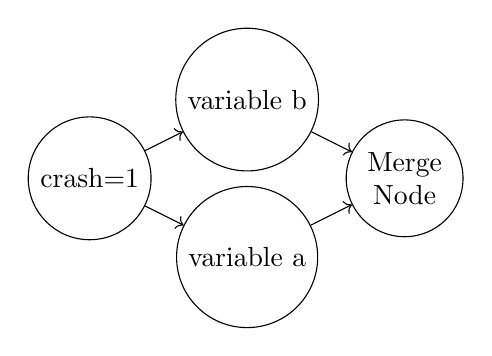
\begin{tikzpicture}
	\node [fill=white, draw=black, shape=circle,align=center] (0) at (0, 0) {crash=1};
	\node [fill=white, draw=black, shape=circle,align=center] (1) at (2, 1) {variable b};
	\node [fill=white, draw=black, shape=circle,align=center] (2) at (2, -1) {variable a};
	\node [fill=white, draw=black, shape=circle,align=center] (3) at (4, 0) {Merge\\Node};
	\draw [fill=none, ->] (0) to (1);
	\draw [fill=none, ->] (0) to (2);
	\draw [fill=none, ->] (1) to (3);
	\draw [fill=none, ->] (2) to (3);
\end{tikzpicture}
  \caption{DAG for the problem with a loop.}
  \label{ex3_dag}


    \end{minipage}
\end{figure}




The above decompositions were all produced using the same recipe and were successfully run with \dagster. These small examples don't motivate large parallel compute, but we are validating our recipes and running them with \dagster\ which is executing these decompostions in parallel. Research is still ongoing into improving the decomposition method that was used to form the above DAG structures.



\clearpage
\section{Model Counting in Parallel - Easy Large Satisfiable Random Formulae}

It is also possible to verify that \dagster\ has steady performance with larger problems, particularly we consider solving large-easy SAT problems which are entirely disjoint and in parallel, similar to the scheme implemented in section \ref{section:section1}.
Particularly it is verified that as the number of large-easy problems increases then the memory that \dagster\ should take in solving these should be less than the size of the CNF file of all those problems combined; and in this way it is verifiable that \dagster\ can solve problems which are larger than the amount of memory on the machine.
This is accomplished by splitting the CNF of the larger problem into parts corresponding to subproblems, which are loaded sequentially and solved in turn in accordance with the DAG.

Particularly a 5MB random-7-SAT problem was generated, and multiple copies of the same problem were concatenated to form a parallel DAG - as previously shown in figure \ref{fig:dag_example4315}).
In this way the maximum size of any subproblem was 5MB, whereas the CNF of the problem would be many multiples of 5MB.

The memory consumed by \dagster\ running these problems against the size of the CNF of these problems for different numbers of cores is shown in figures \ref{fig:memory_consumption}.
From figure \ref{fig:memory_consumption} we can see that the memory used is a barely a fraction of the size of the CNF, which doesn't vary considerably with the number of cores.
From this experiment it can be verified that \dagster\ can tackle problems which are large with respect to the available memory.

The invocation to run these experiments is to be found by executed the following command within the code repository:

\begin{verbatim}
~/summer1819/Benchmarks/cnf_concatenator/runme.sh
\end{verbatim}


   \begin{figure}[h]
        \centering
		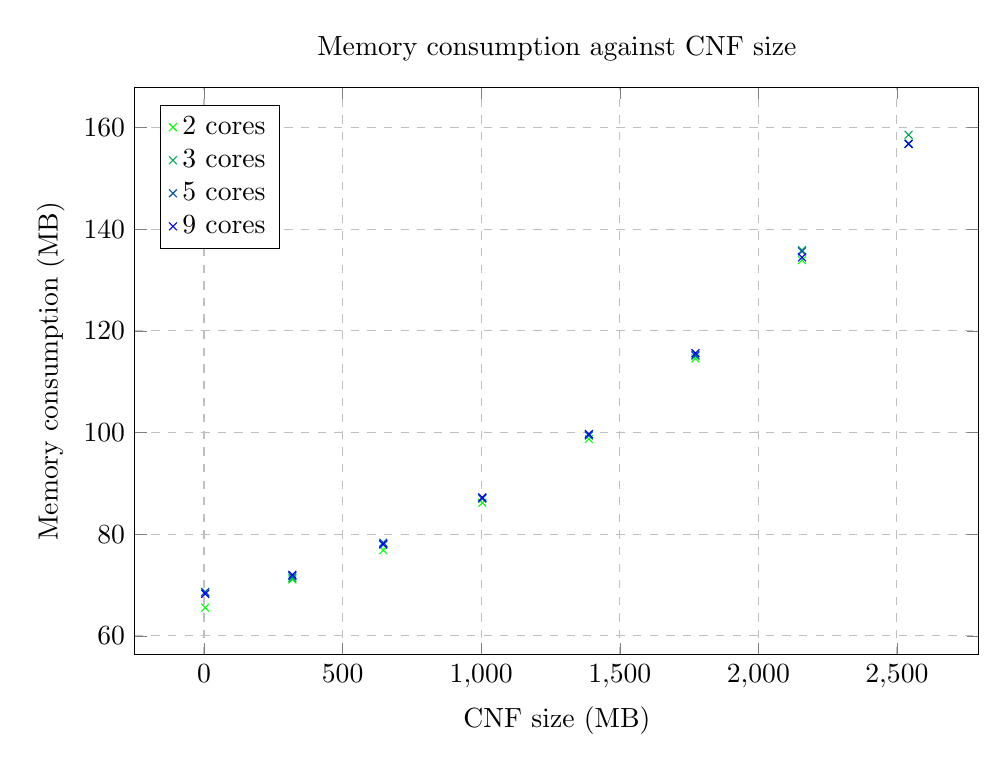
\begin{tikzpicture}
		\begin{axis}[
			title={Memory consumption against CNF size},
			xlabel={CNF size (MB)},
			ylabel={Memory consumption (MB)},
			%xmin=0, xmax=0.25,
			%ymin=10.00, ymax=100000.00,
			%ymode=log,
			%xmode=log,
			%xtick={0,0.05,0.1,0.15,0.2,0.25},
			%ytick={0,20,40,60,80,100},
			%yticklabel=$\pgfmathprintnumber{\tick}\%$,
			legend pos=north west,
			ymajorgrids=true,
			xmajorgrids=true,
			grid style=dashed,
			xticklabel style={/pgf/number format/fixed},
			width = 350,
			height = 250
		]



\addplot[color=blue!0!green,only marks,mark=x] coordinates {
(4.1669921875,65.5703125)(318.771484375,71.09375)(646.669921875,76.87890625)(1004.0185546875,86.203125)(1388.5263671875,98.7421875)(1773.03515625,114.58984375)(2157.5439453125,133.93359375)(2542.052734375,156.85546875)
}node[pos=0.8](endofplotsquare){} ;
\addlegendentry{2 cores}
\addplot[color=blue!33!green,only marks,mark=x] coordinates {
(4.1669921875,68.35546875)(318.771484375,71.37109375)(646.669921875,77.9296875)(1004.0185546875,87.015625)(1388.5263671875,99.54296875)(1773.03515625,115.32421875)(2157.5439453125,135.91015625)(2542.052734375,158.578125)
}node[pos=0.8](endofplotsquare){} ;
\addlegendentry{3 cores}
\addplot[color=blue!67!green,only marks,mark=x] coordinates {
(4.1669921875,68.64453125)(318.771484375,71.76171875)(646.669921875,78.34765625)(1004.0185546875,87.07421875)(1388.5263671875,99.421875)(1773.03515625,115.16015625)(2157.5439453125,135.640625)(2542.052734375,156.77734375)
}node[pos=0.8](endofplotsquare){} ;
\addlegendentry{5 cores}
\addplot[color=blue!100!green,only marks,mark=x] coordinates {
(4.1669921875,68.26171875)(318.771484375,72.02734375)(646.669921875,78.0703125)(1004.0185546875,87.23828125)(1388.5263671875,99.71875)(1773.03515625,115.62109375)(2157.5439453125,134.48046875)(2542.052734375,156.8046875)
}node[pos=0.8](endofplotsquare){} ;
\addlegendentry{9 cores}





		\end{axis}
		\end{tikzpicture}
		%\vspace{-18pt}
  \caption{\dagster\ memory consumption for conjunctions of large-easy problems against core count.\label{fig:memory_consumption}}
    \end{figure}



\renewcommand{\refname}{\spacedlowsmallcaps{References}} % For modifying the bibliography heading
\bibliographystyle{unsrt}
\bibliography{bib.bib} % The file containing the bibliography
\end{document}
